\documentclass[a4paper,12pt]{report}

\usepackage{cmap}
\usepackage[T2A]{fontenc}
\usepackage[utf8]{inputenc}
\usepackage[english,russian]{babel}
\usepackage{listings}
\usepackage{amsmath}
\usepackage{float}
\usepackage{csquotes}
\usepackage{mathtools}
\usepackage{hyphenat}
\usepackage{amsfonts}
\usepackage{upgreek}

\usepackage{xcolor}
\usepackage{hyperref}

\usepackage{graphicx}
\graphicspath{ {./images/} }

\definecolor{dkgreen}{rgb}{0,0.6,0}
\definecolor{gray}{rgb}{0.5,0.5,0.5}
\definecolor{mauve}{rgb}{0.58,0,0.82}

\lstset{
    language=Python,                 % выбор языка для подсветки (здесь это С)
    basicstyle=\small\sffamily, % размер и начертание шрифта для подсветки кода
    numbers=left,               % где поставить нумерацию строк (слева\справа)
    numberstyle=\tiny,           % размер шрифта для номеров строк
    stepnumber=1,                   % размер шага между двумя номерами строк
    numbersep=5pt,                % как далеко отстоят номера строк от подсвечиваемого кода
    aboveskip=3mm,
    belowskip=3mm,
    showstringspaces=false,
    columns=flexible,
    captionpos=b, 
    basicstyle={\small\ttfamily},
    numbers=left,
    numberstyle=\tiny\color{gray},
    keywordstyle=\color{blue},
    commentstyle=\color{mauve},
    stringstyle=\color{dkgreen},
    breaklines=true,
    breakatwhitespace=true,
    tabsize=3
}

\title{Лабораторная работа №12\\GNU Radio}
\author{Кобыжев Александр}
\date{\today}

\begin{document}

\maketitle
\tableofcontents
\listoffigures

\maketitle

\chapter{Передача сигнала}

На данном этапе нашей задачей является передача сигнала \texttt{QPSK}. Для этого мы генерируем поток битов и моделируем его на сложное созвездие, используя при этом блоки \texttt{Constellation Modulator} и блок \texttt{Constellation Rect}. 

Рассмотрим получившуюся схему из модулей и график ниже, который визуализирует генерацию различных значений избыточной пропускной способности. 

\begin{figure}[H]
        \centering
        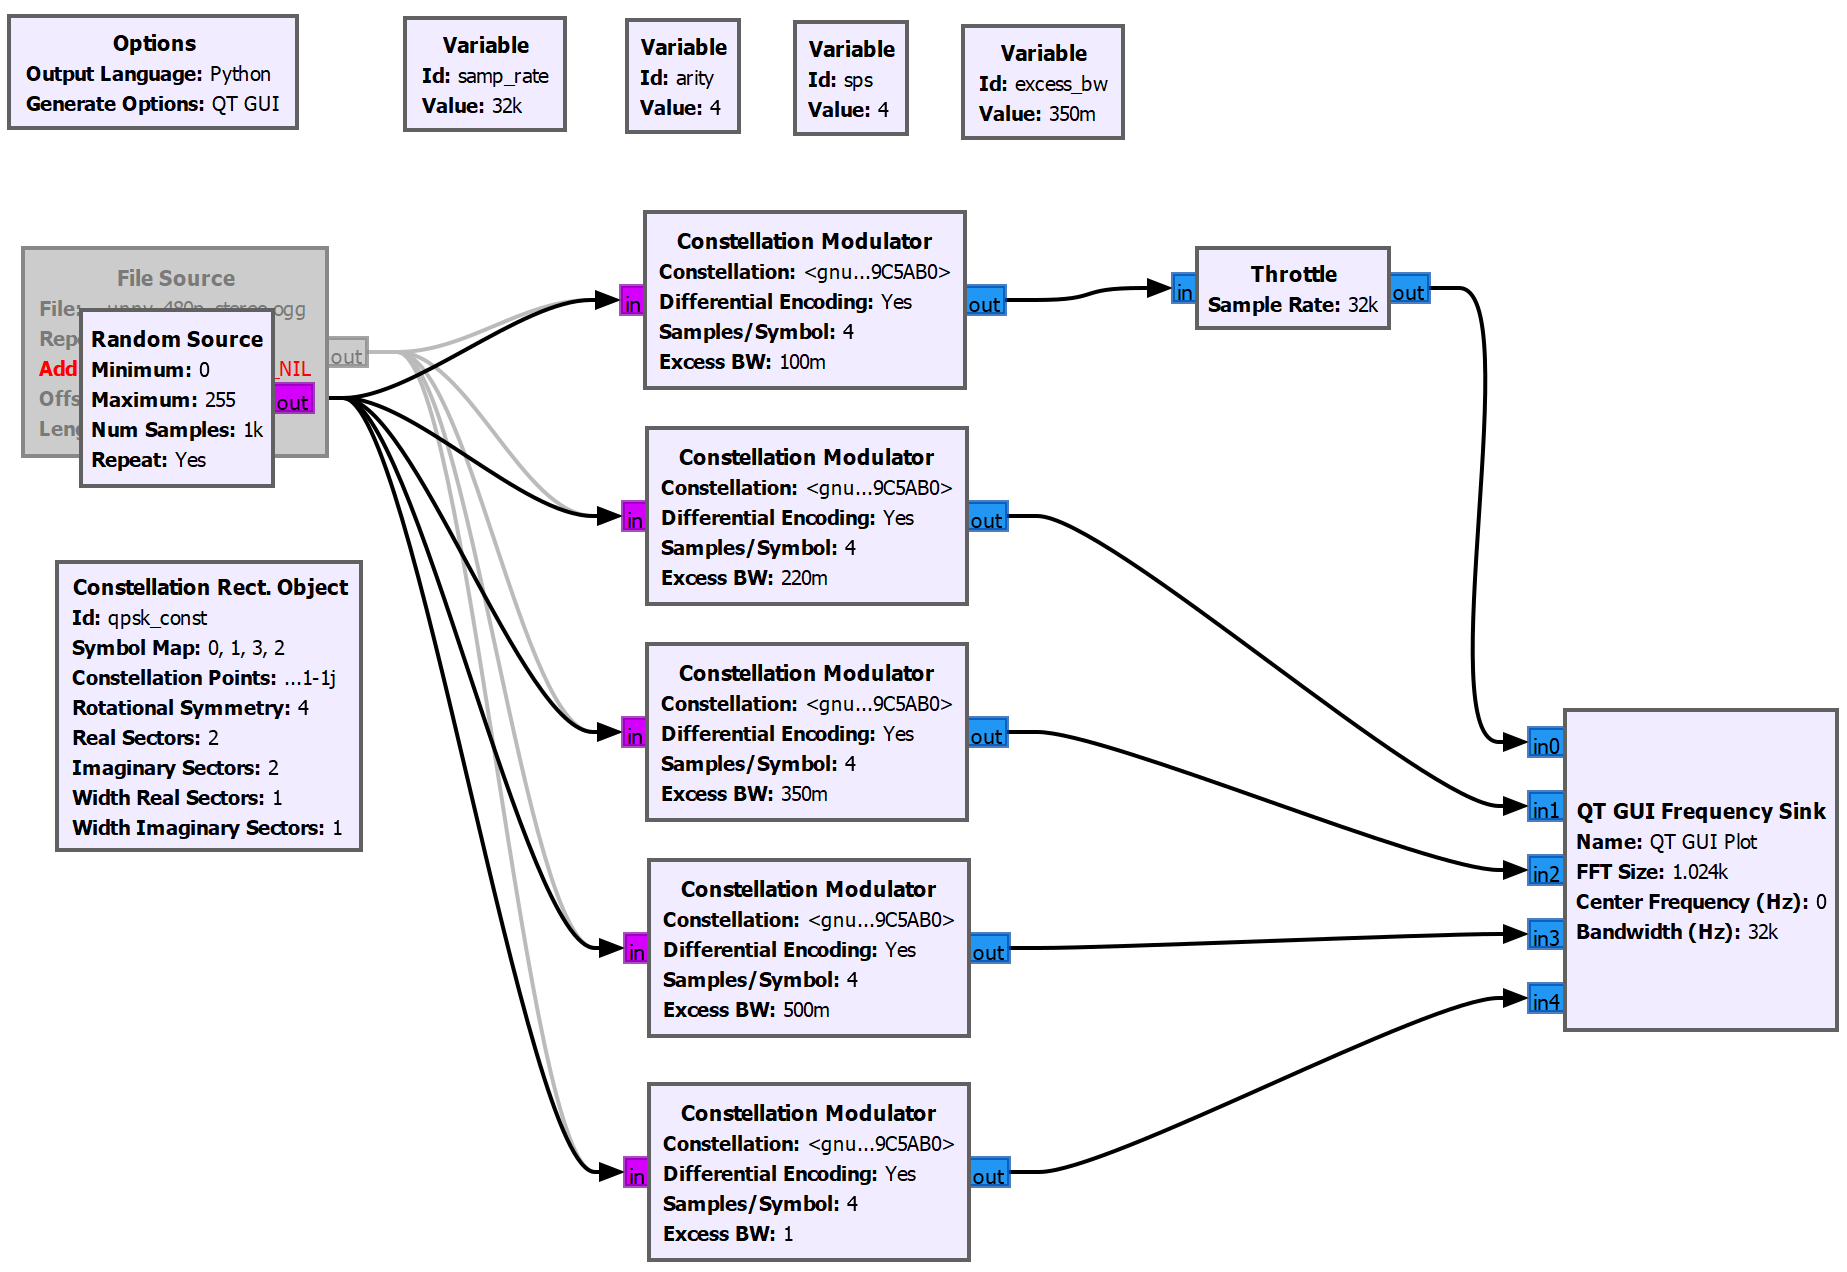
\includegraphics[width=1.0\textwidth]{lab12_fig1_1.png}
        \caption{mpsk\_rrc\_rolloff схема}
        \label{fig:lab11_fig3_1}
\end{figure}

\begin{figure}[H]
        \centering
        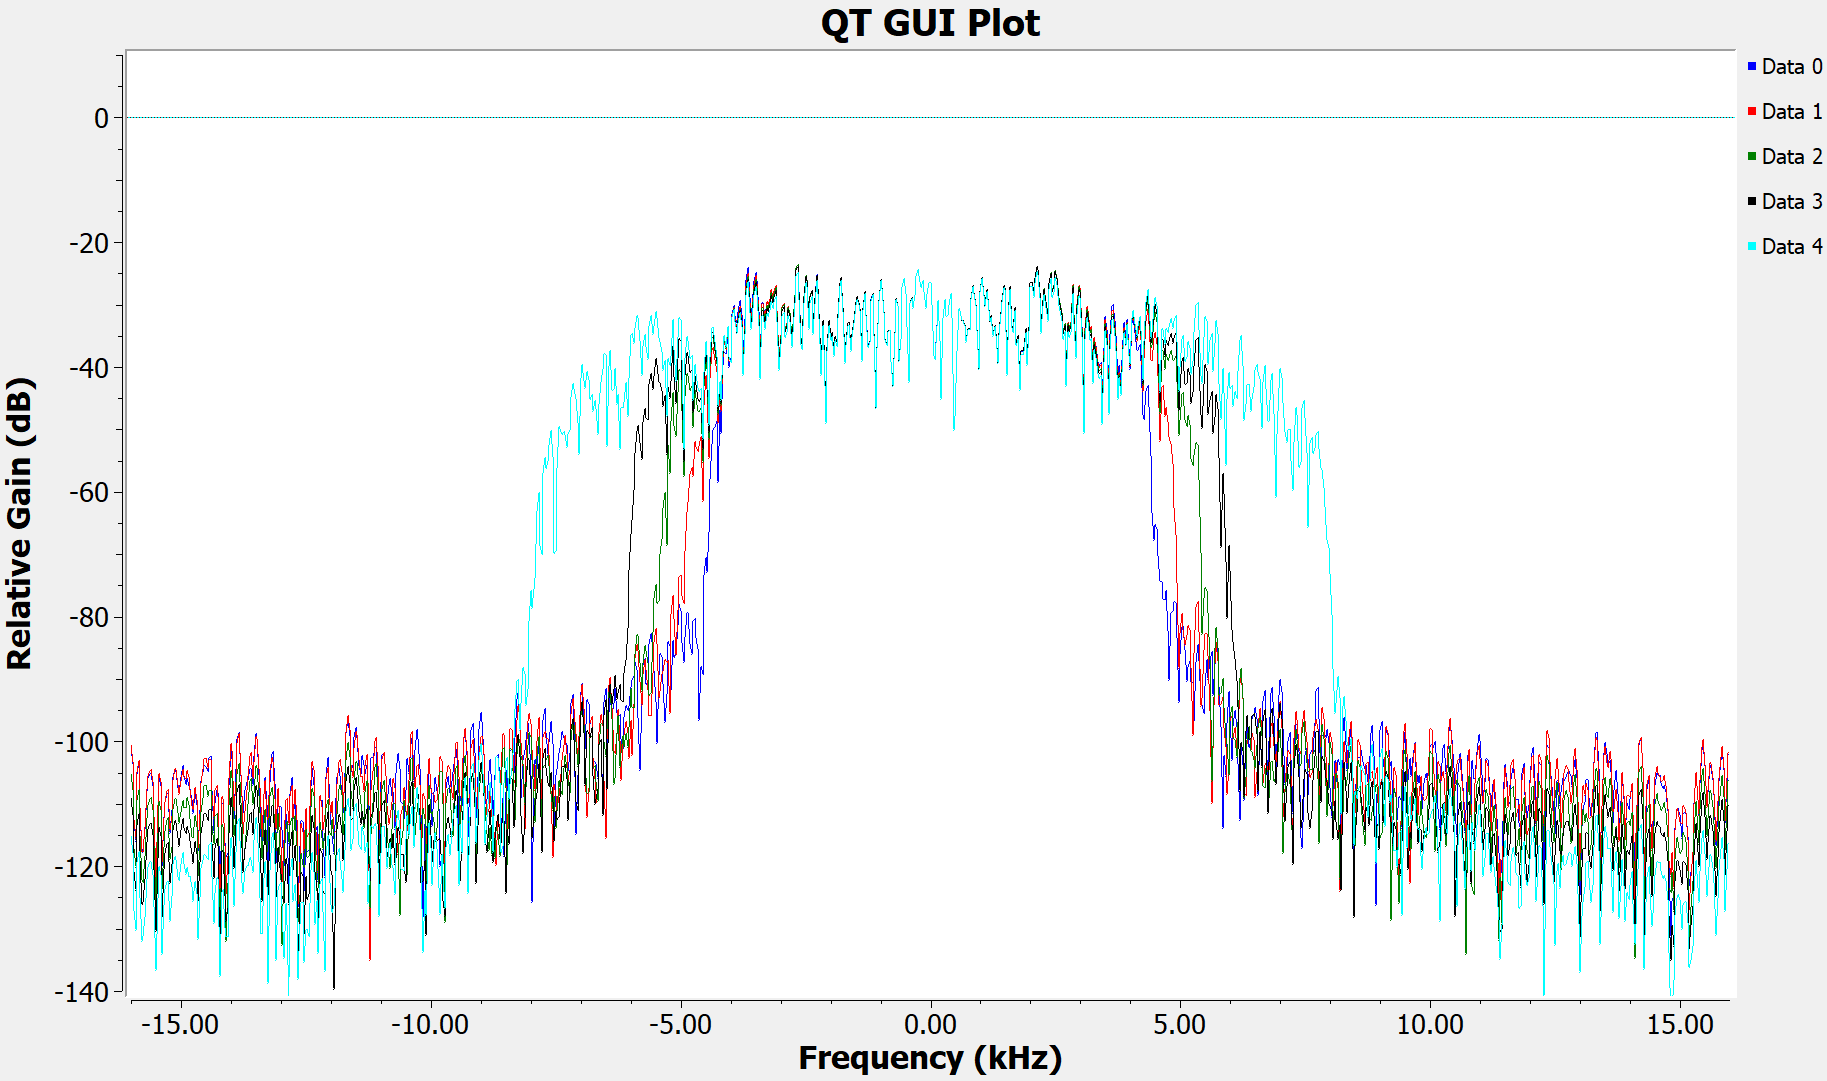
\includegraphics[width=1.0\textwidth]{lab12_fig1_2.png}
        \caption{Визуализация генерации данных}
        \label{fig:lab12_fig1_2}
\end{figure}

Теперь рассмотрим пример потокового графа, который передает созвездие \texttt{QPSK}. Он отображает как передаваемый сигнал, так и часть цепи приемника во времени, частоте и диаграмме созвездия. Получившаяся схема выглядит следующим образом:

\begin{figure}[H]
        \centering
        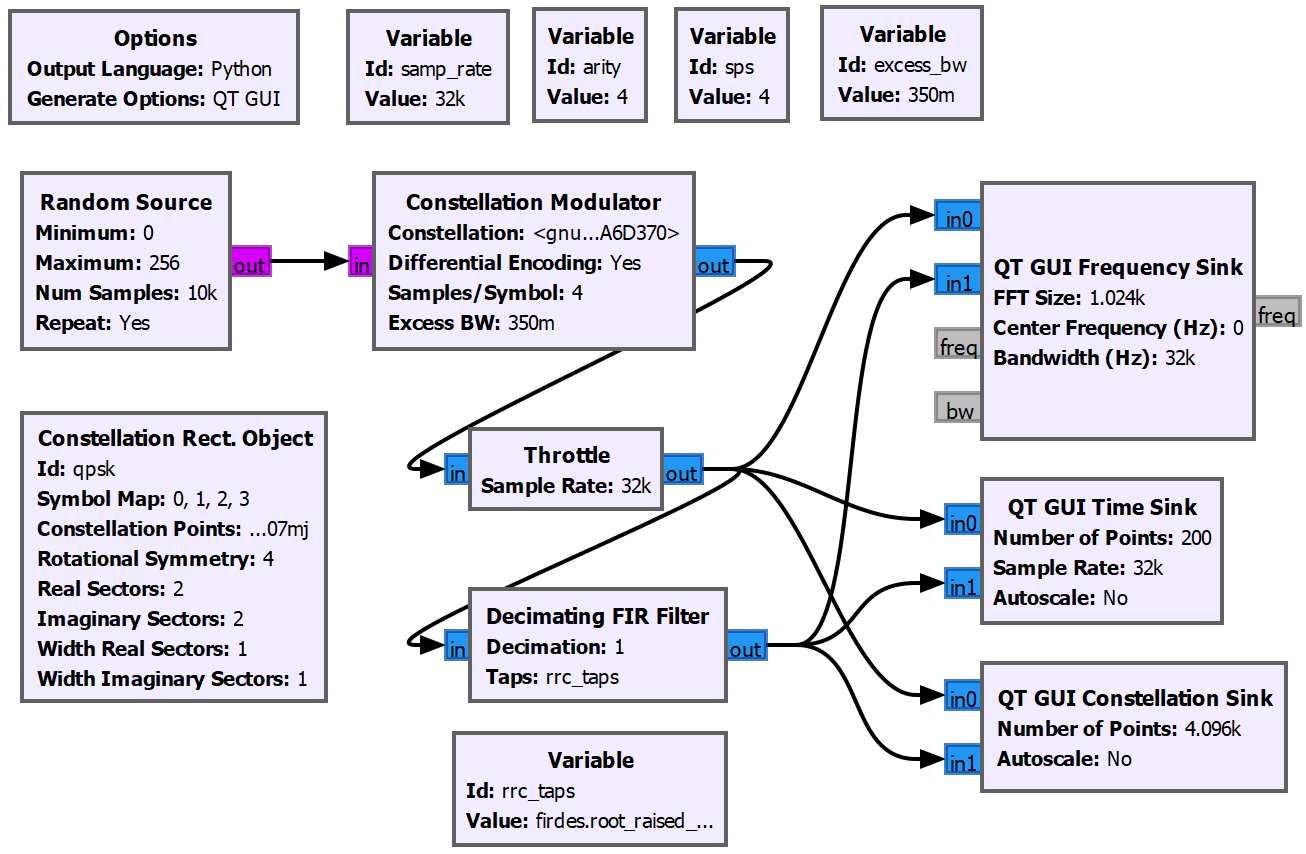
\includegraphics[width=1.0\textwidth]{lab12_fig1_3.png}
        \caption{mpsk\_stage1 схема}
        \label{fig:lab12_fig1_3}
\end{figure}

На графике созвездия мы видим эффекты повышающей дискретизации (то есть генерирование 4 выборок на символ) и процесса фильтрации. Фильтр \texttt{RRC} добавляет преднамеренные собственные помехи, известные как межсимвольные помехи (\texttt{ISI}). Благодаря уменьшению внеполосных излучений наш сигнал теперь остается в пределах полосы пропускания нашего канала.

\begin{figure}[H]
        \centering
        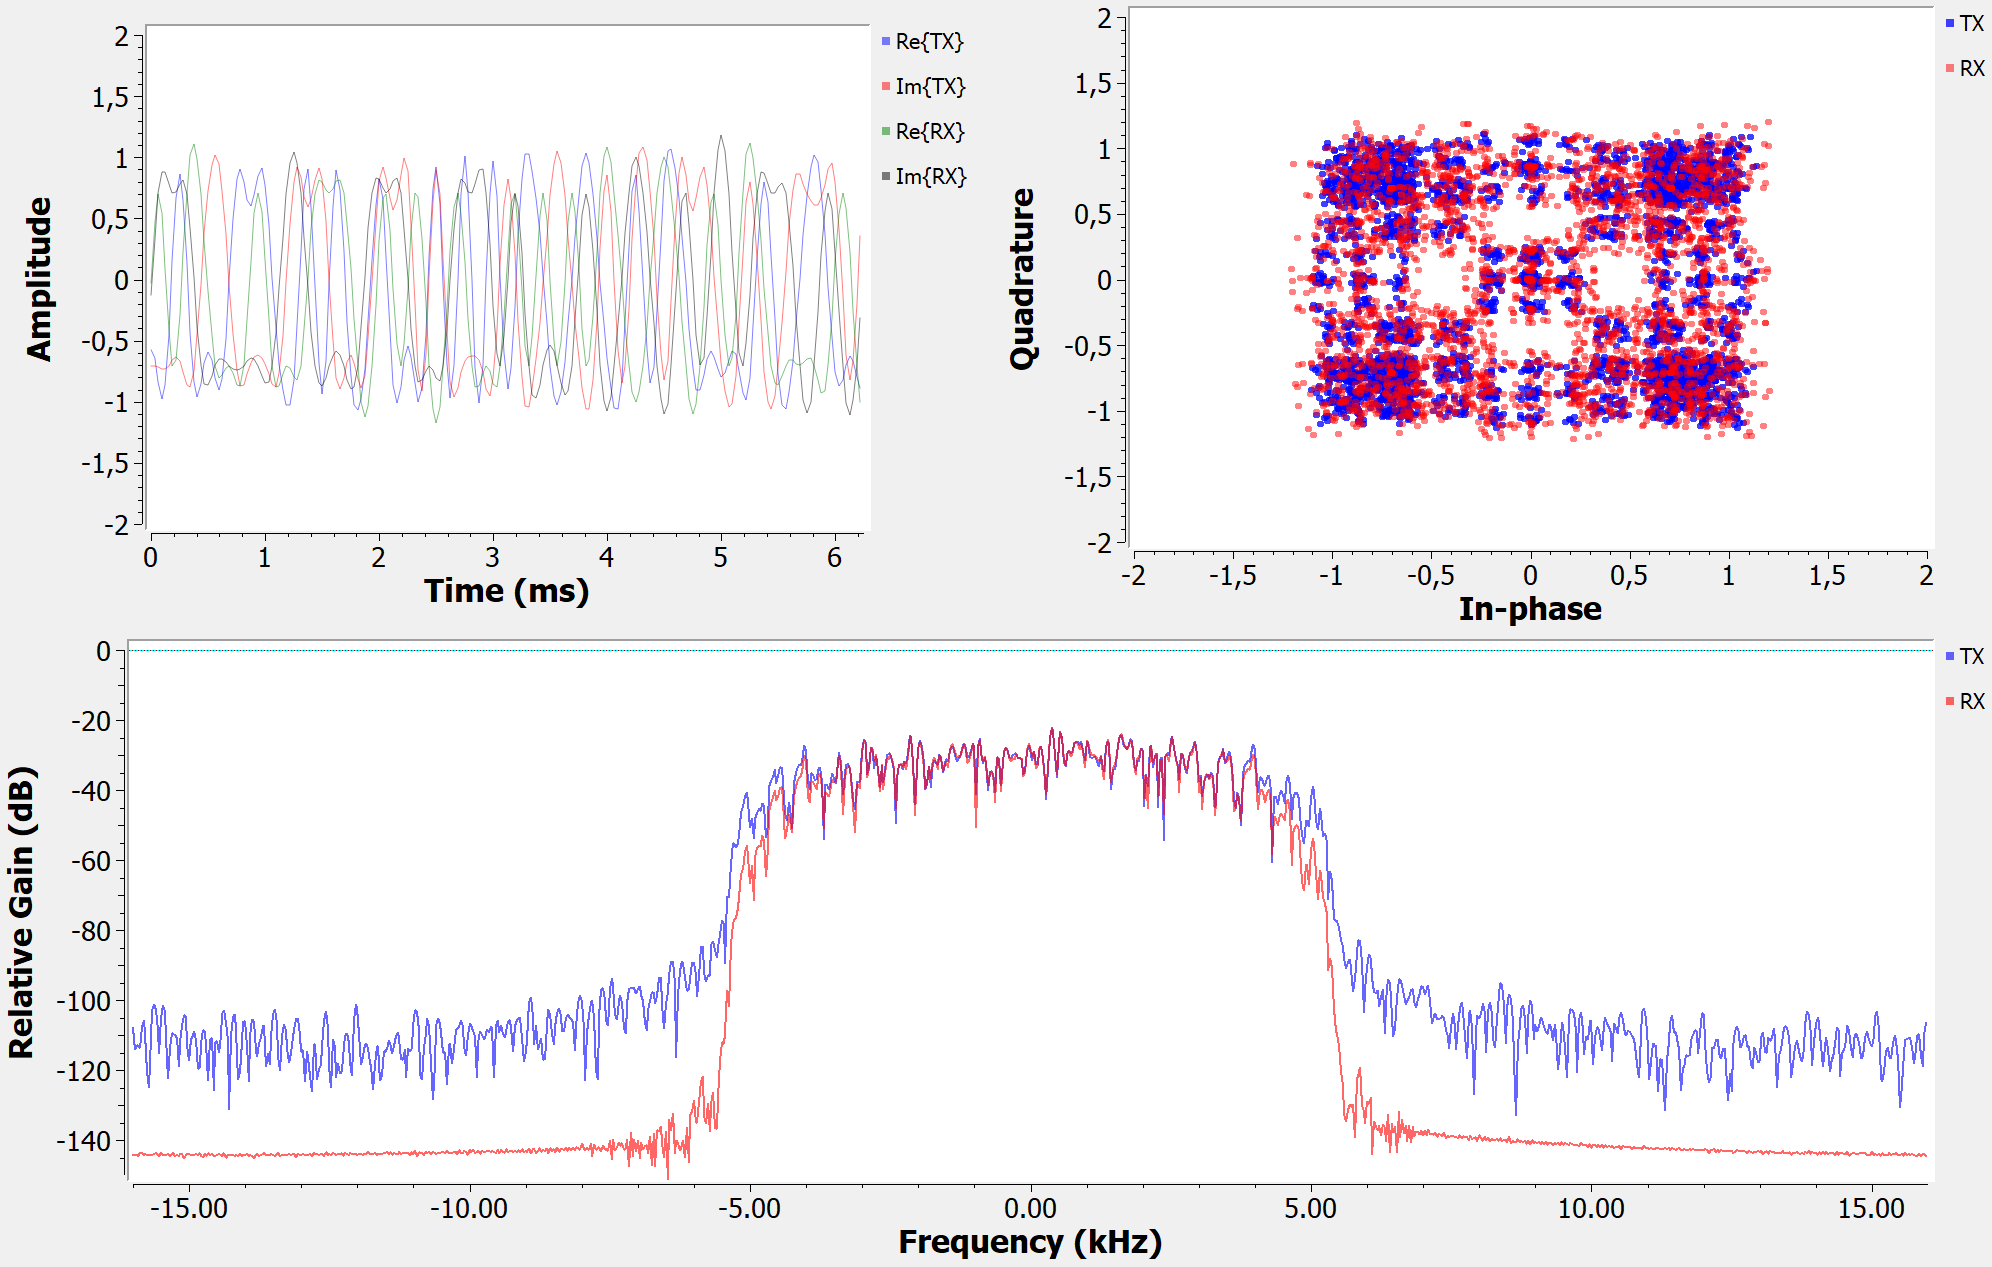
\includegraphics[width=1.0\textwidth]{lab12_fig1_4.png}
        \caption{Визуализация генерации данных для схемы mpsk\_stage1}
        \label{fig:lab12_fig1_4}
\end{figure}

\chapter{Добавление искажений канала}

Теперь на данном этапе рассмотрим влияние канала, а также искажение сигнала во время передачи, и когда мы видим его в приёмнике. Для этого мы будем использовать блок \texttt{Channel Model}, который позволит смоделировать проблему появления шума, а также различие clock'ов, которые определяют частоту радиомодулей. Благодаря этому мы можем поиграть с эффектами шума, сдвига частоты и временного сдвига. Для следующего графика выставлены следующие параметры: шум - 0,2, смещение частоты - 0,025, смещение времени - 1,0005.

\begin{figure}[H]
        \centering
        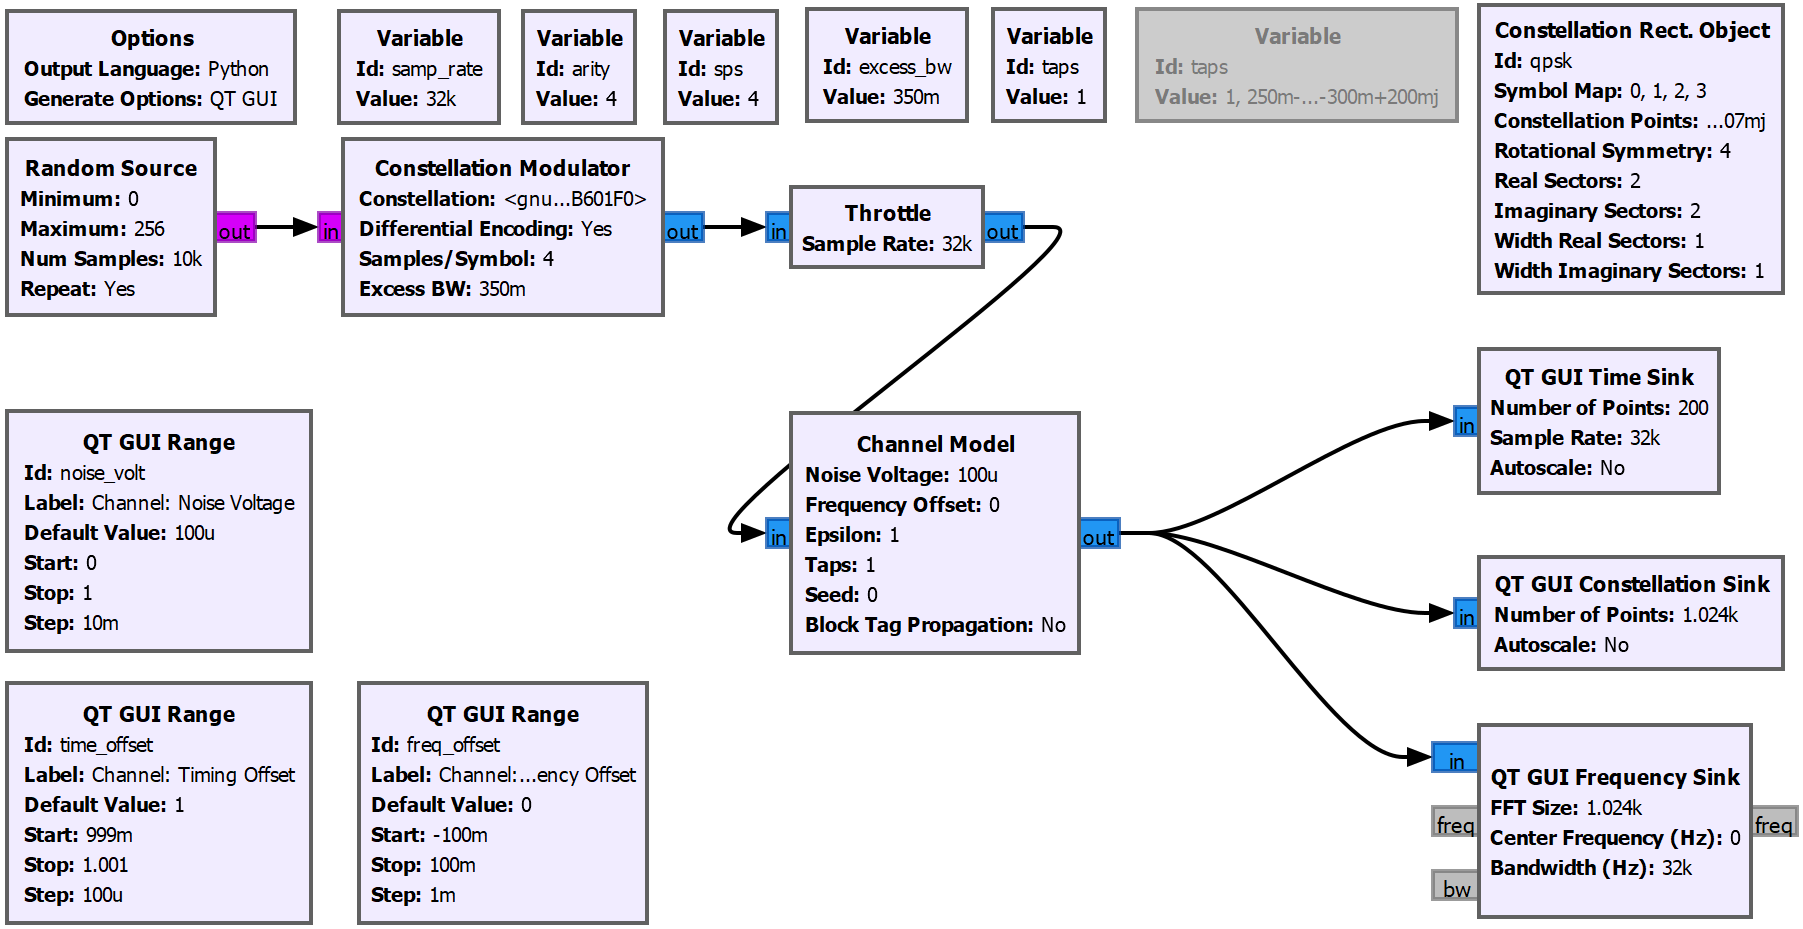
\includegraphics[width=1.0\textwidth]{lab12_fig2_1.png}
        \caption{mpsk\_stage2 схема}
        \label{fig:lab12_fig2_1}
\end{figure}

\begin{figure}[H]
        \centering
        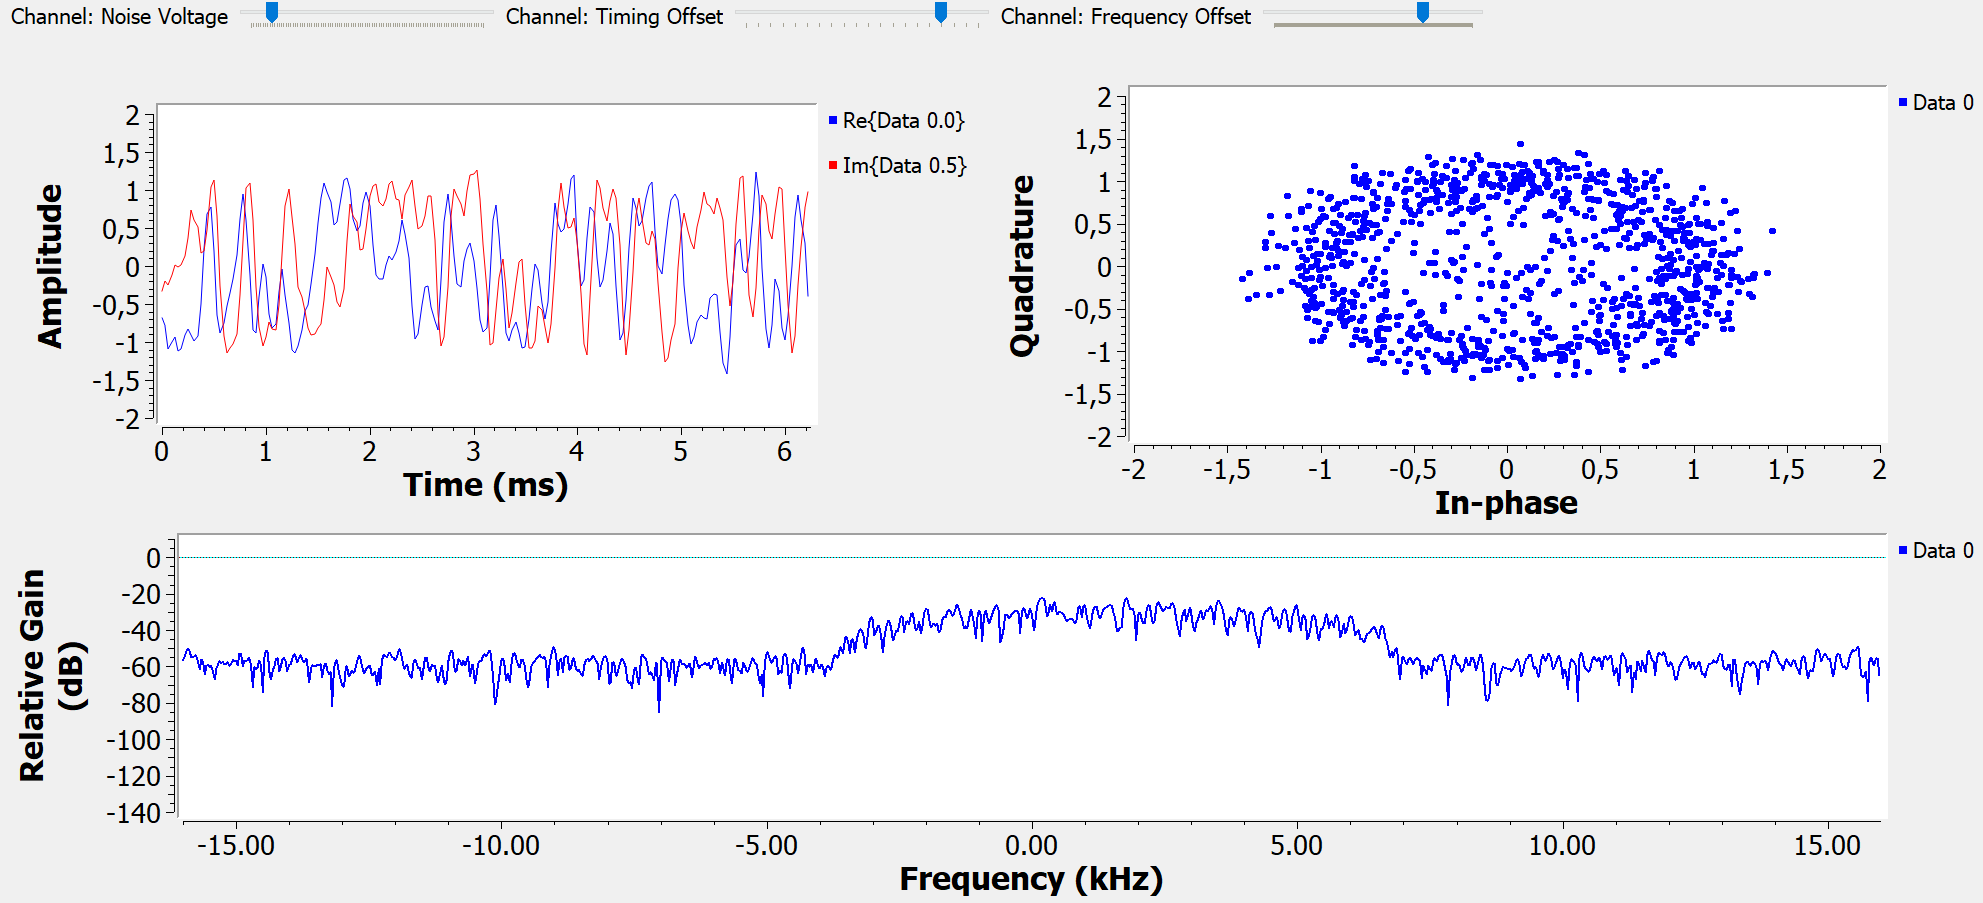
\includegraphics[width=1.0\textwidth]{lab12_fig2_2.png}
        \caption{Визуализация генерации данных}
        \label{fig:lab12_fig2_2}
\end{figure}

В итоге мы получили график созвездия, выглядящий гораздо хуже, чем тот, что был на первом этапе.

\chapter{Временное восстановление}

\section{Алгоритм восстановления многофазных clock'ов}

Теперь рассмотрим процесс восстановления и начнем с временного восстановления. Мы пытаемся найти наилучшее время для дискретизации входящих сигналов, что позволит максимизировать отношение сигнал/шум (\texttt{SNR}) каждой выборки, а также уменьшить влияние межсимвольных помех (\texttt{ISI}). Для того, чтобы проиллюстрировать проблему \texttt{ISI} на примере потокового графа, просто создадим четыре отдельных символа из единиц в потоке, а затем отфильтруем их.

\begin{figure}[H]
        \centering
        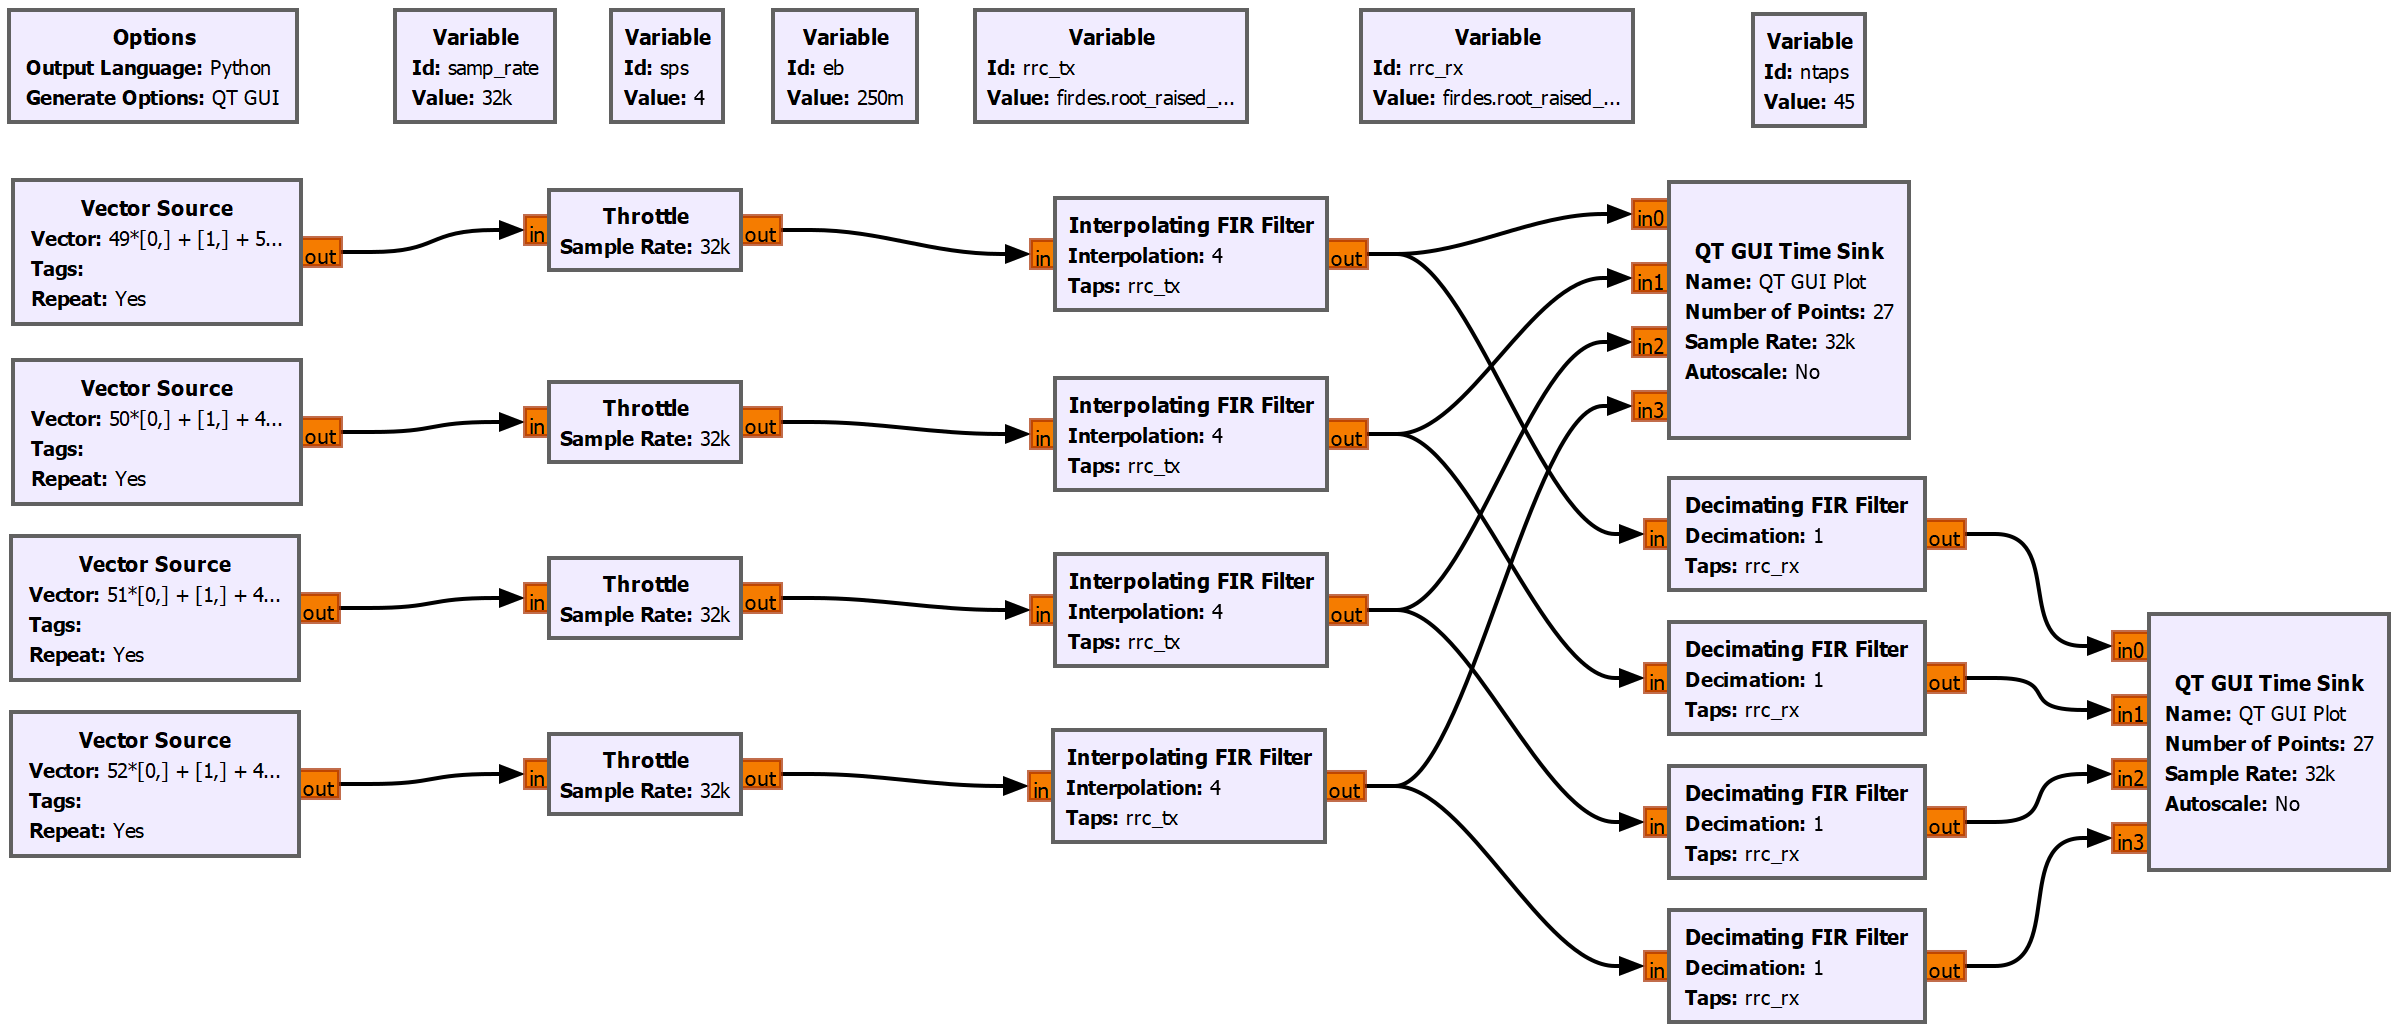
\includegraphics[width=1.0\textwidth]{lab12_fig3_1.png}
        \caption{symbol\_sampling схема}
        \label{fig:lab12_fig3_1}
\end{figure}

\begin{figure}[H]
        \centering
        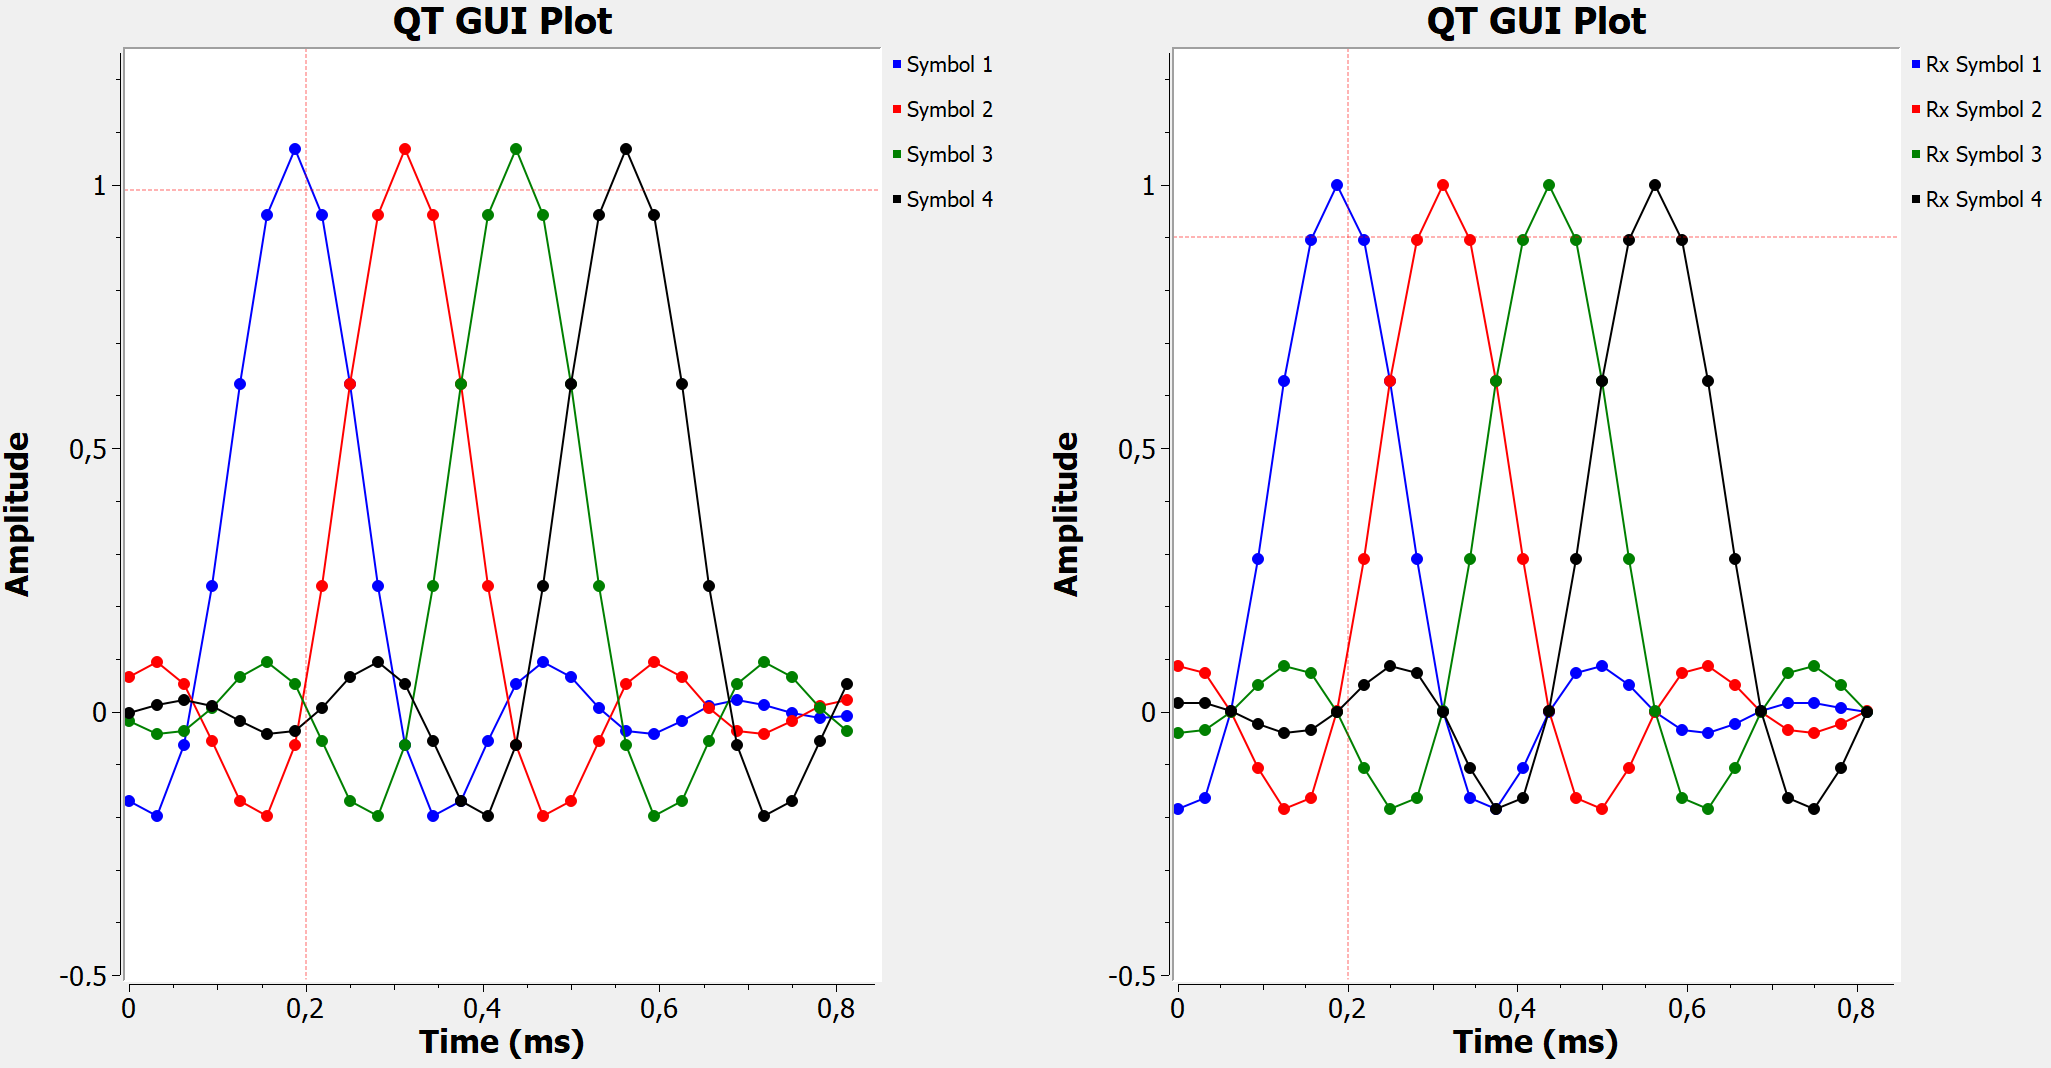
\includegraphics[width=1.0\textwidth]{lab12_fig3_2.png}
        \caption{Визуализация потокового графа}
        \label{fig:lab12_fig3_2}
\end{figure}

Это моделирование позволяет нам легко настраивать такие вещи, как количество выборок на символ, избыточную полосу пропускания фильтров RRC и количество ответвлений. После этого мы можем поиграть с этими различными значениями, чтобы увидеть, как они влияют на поведение точки выборки.

Теперь рассмотрим влияния разных clock'ов на точки выборки между передатчиком и приёмником. Для модуляции этого, мы добавлям \texttt{Resampler}, который немного регулирует время выборки символа между переданным сигналом и приёмником.

\begin{figure}[H]
        \centering
        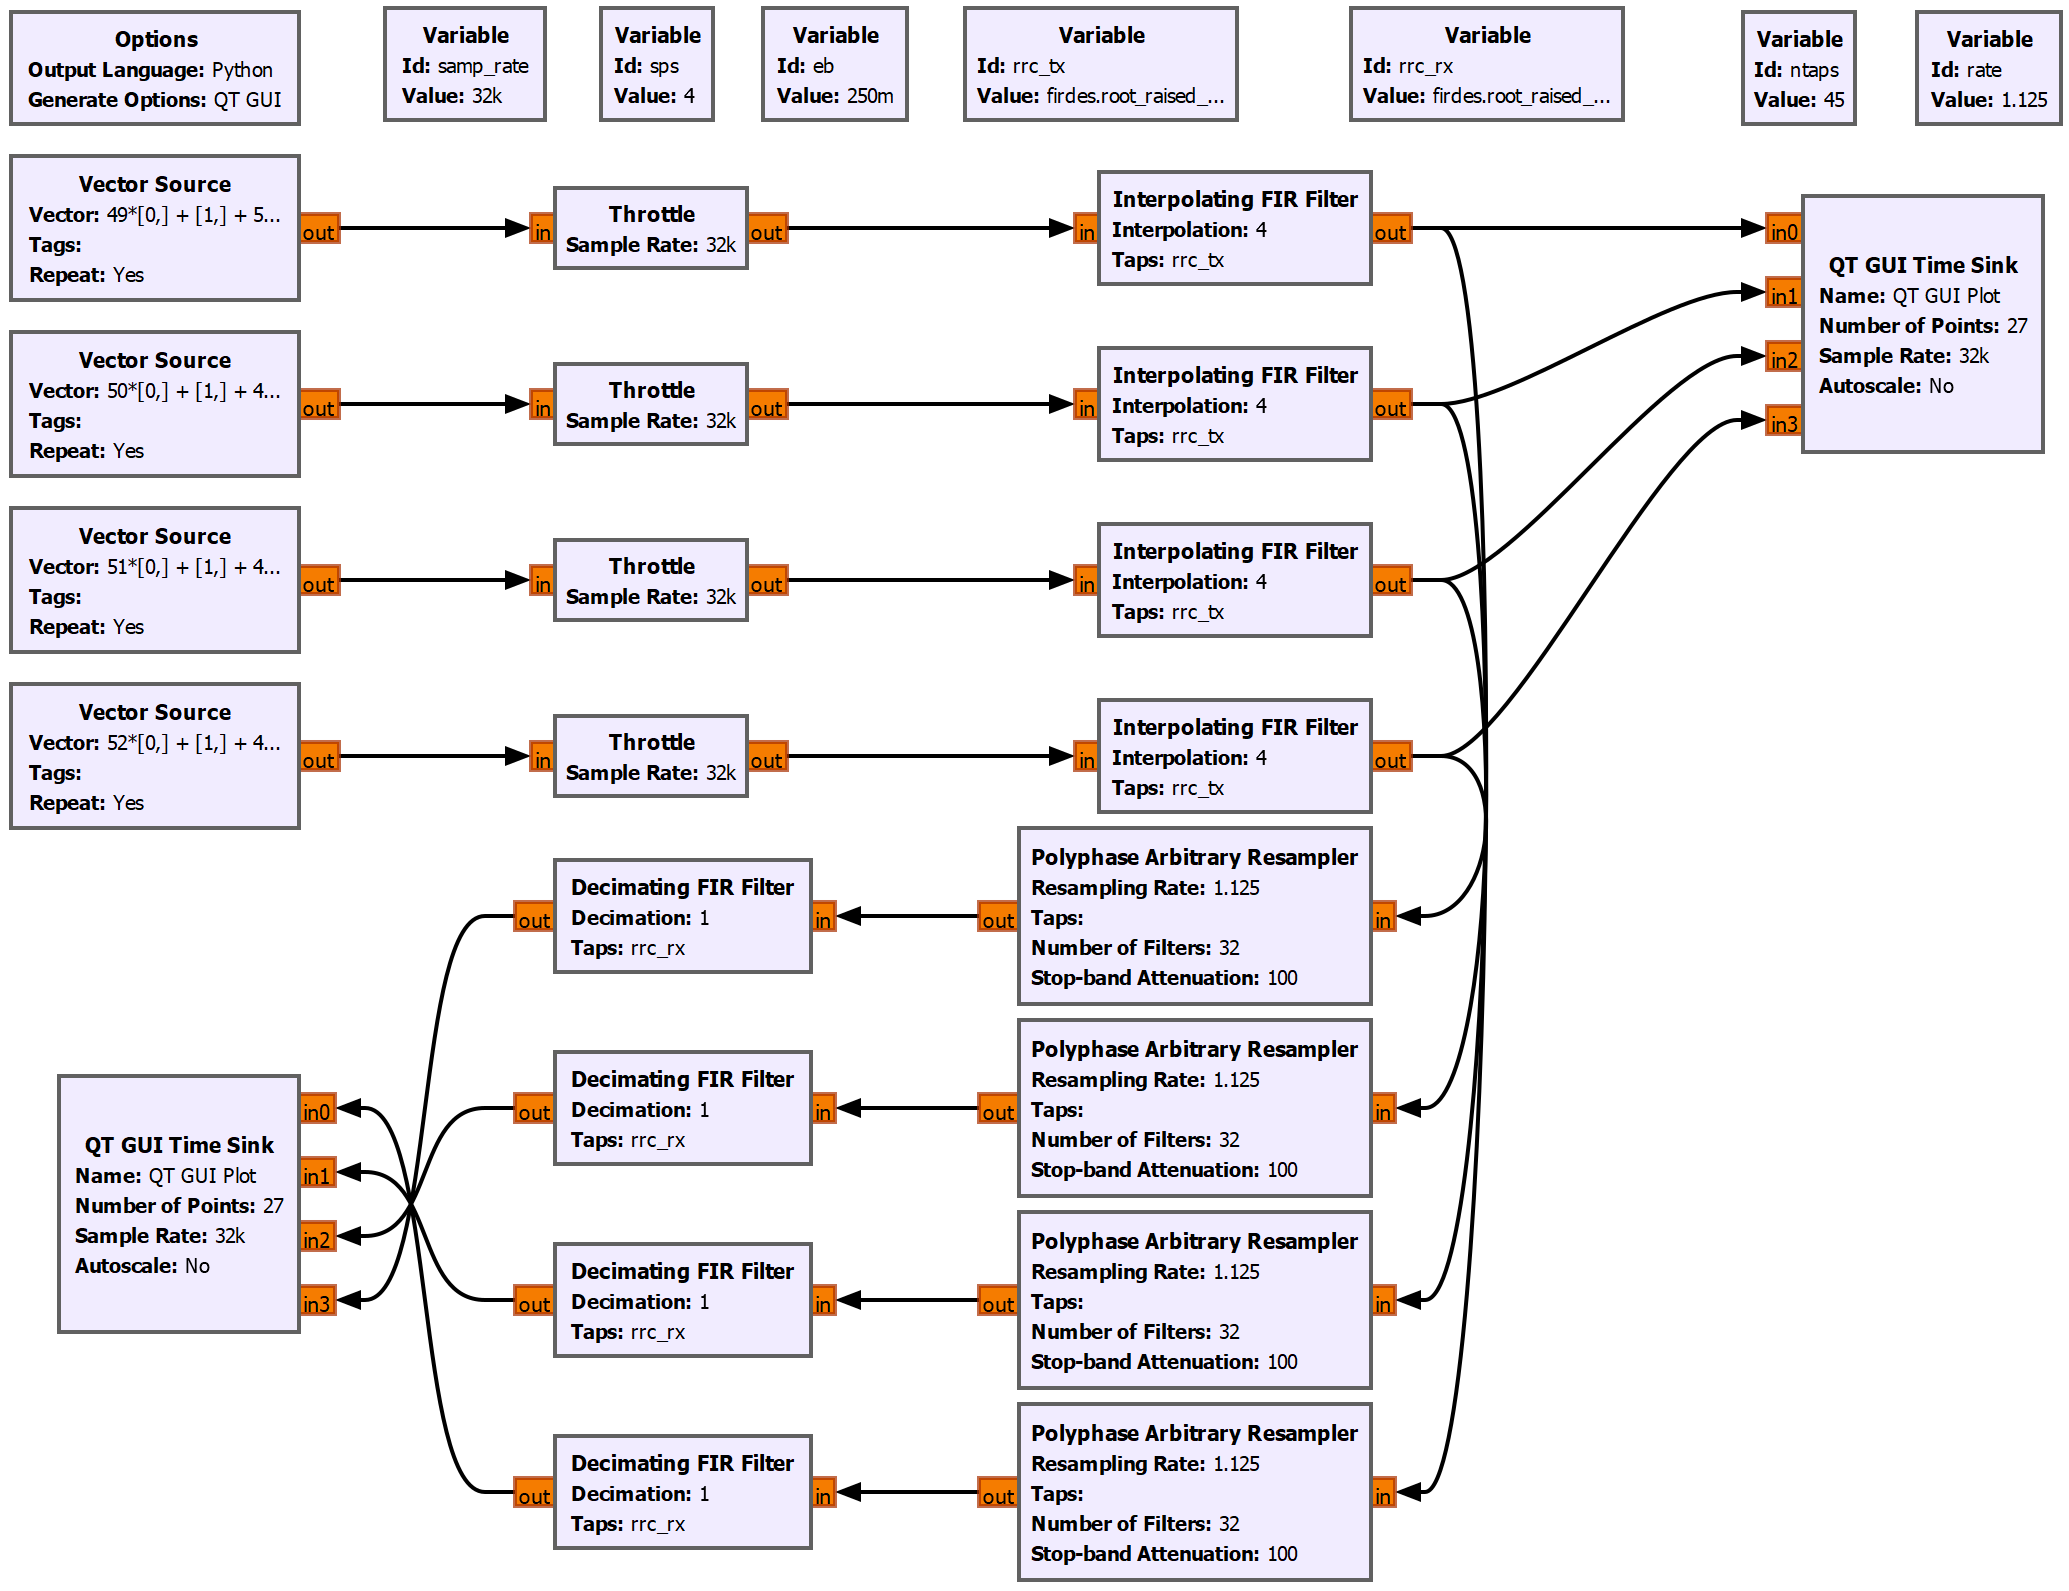
\includegraphics[width=1.0\textwidth]{lab12_fig3_3.png}
        \caption{symbol\_sampling\_diff схема}
        \label{fig:lab12_fig3_3}
\end{figure}

\begin{figure}[H]
        \centering
        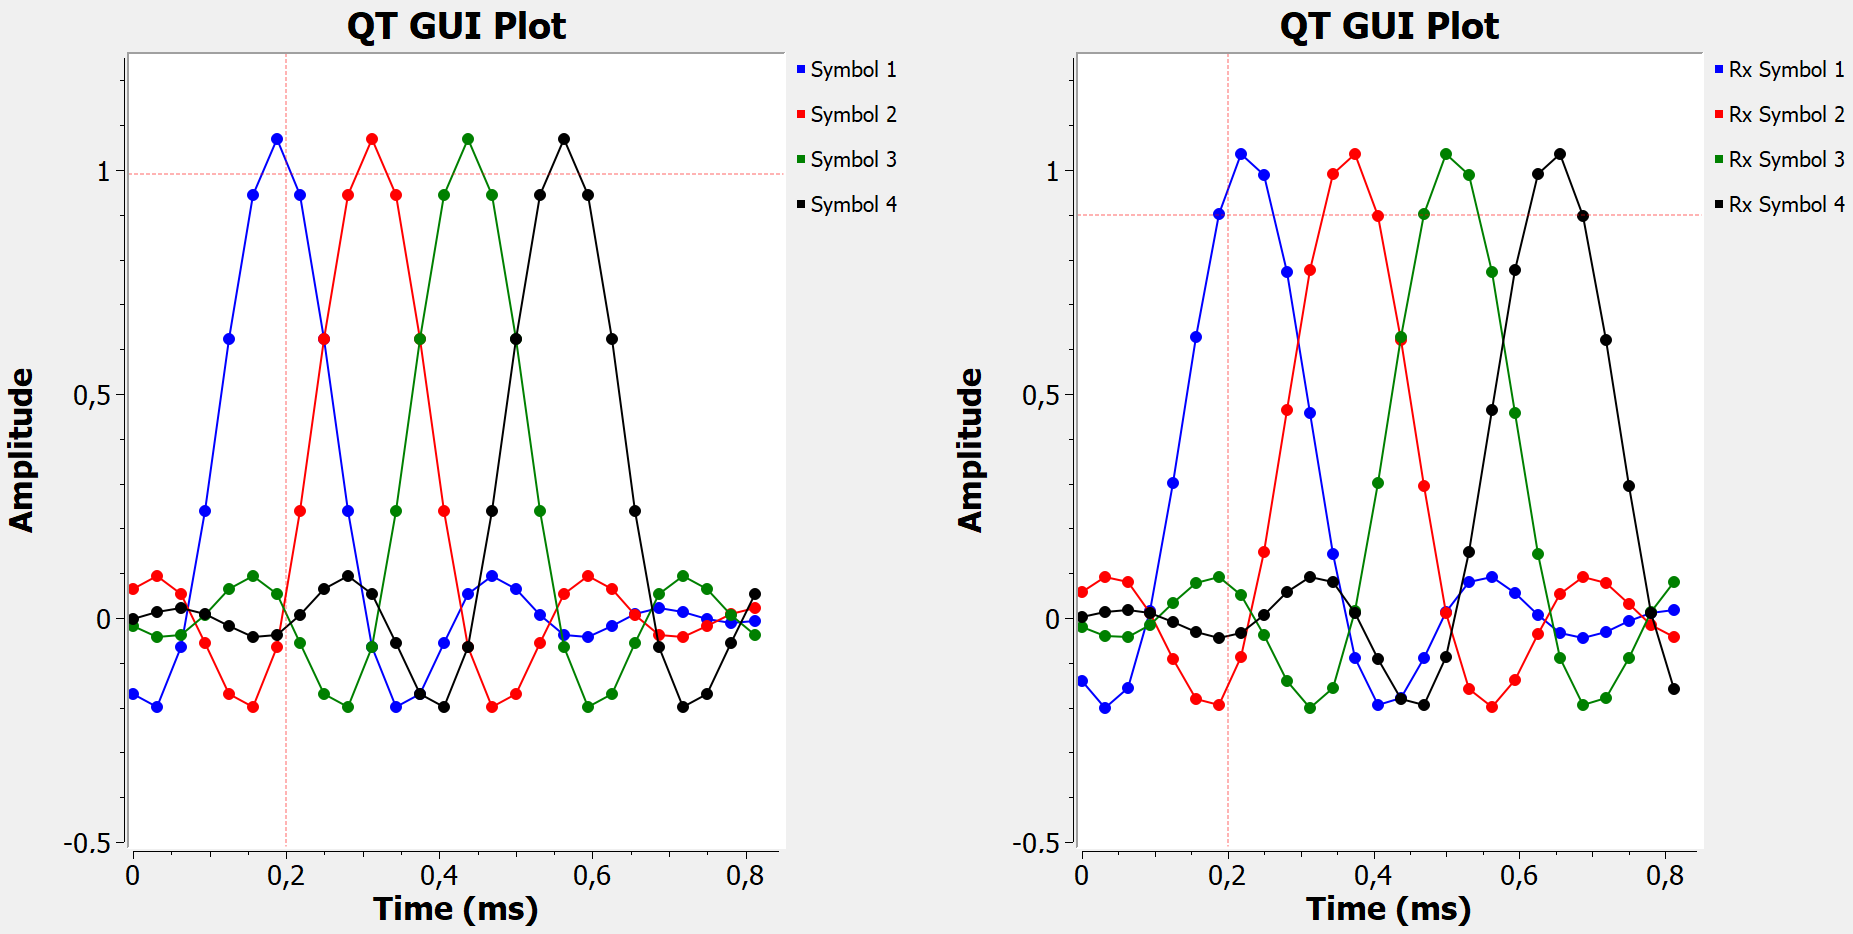
\includegraphics[width=1.0\textwidth]{lab12_fig3_4.png}
        \caption{Визуализация потокового графа}
        \label{fig:lab12_fig3_4}
\end{figure}

\section{Подробная информация о блоке синхронизации многофазных clock'ов}

Блок синхронизации многофазных clock'ов, во-первых, выполняет восстановление clock'ов. Во-вторых, он выполняет согласованный фильтр приёмника для устранения проблемы \texttt{ISI}. В-третьих, он выполняет понижающую дискретизацию сигнала и производит выборки со скоростью 1 sps.

Блок работает, вычисляя первый дифференциал входящего сигнала, который будет связан с его смещением тактовой частоты. Фильтр разности ([-1, 0, 1]) генерирует дифференциал символа, и выходной сигнал этого фильтра в правильной точке выборки равен 0. Затем мы можем инвертировать этот оператор и вместо этого сказать, что когда выход дифференциального фильтра равен 0, то мы нашли оптимальную точку выборки.

\begin{figure}[H]
        \centering
        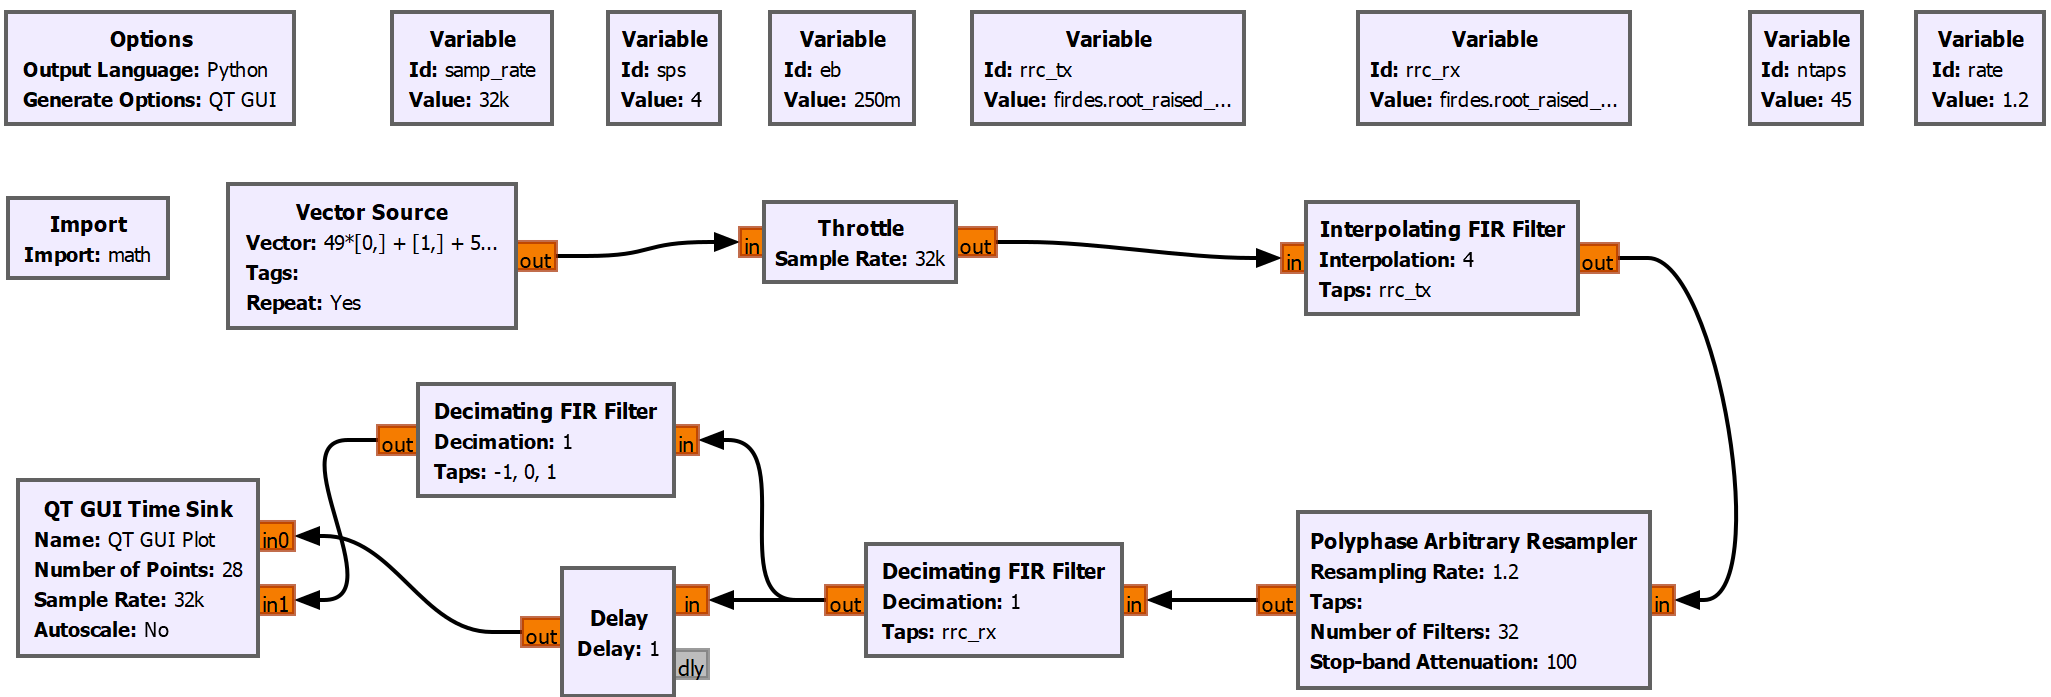
\includegraphics[width=1.0\textwidth]{lab12_fig3_5.png}
        \caption{symbol\_differential\_filter схема}
        \label{fig:lab12_fig3_5}
\end{figure}

\begin{figure}[H]
        \centering
        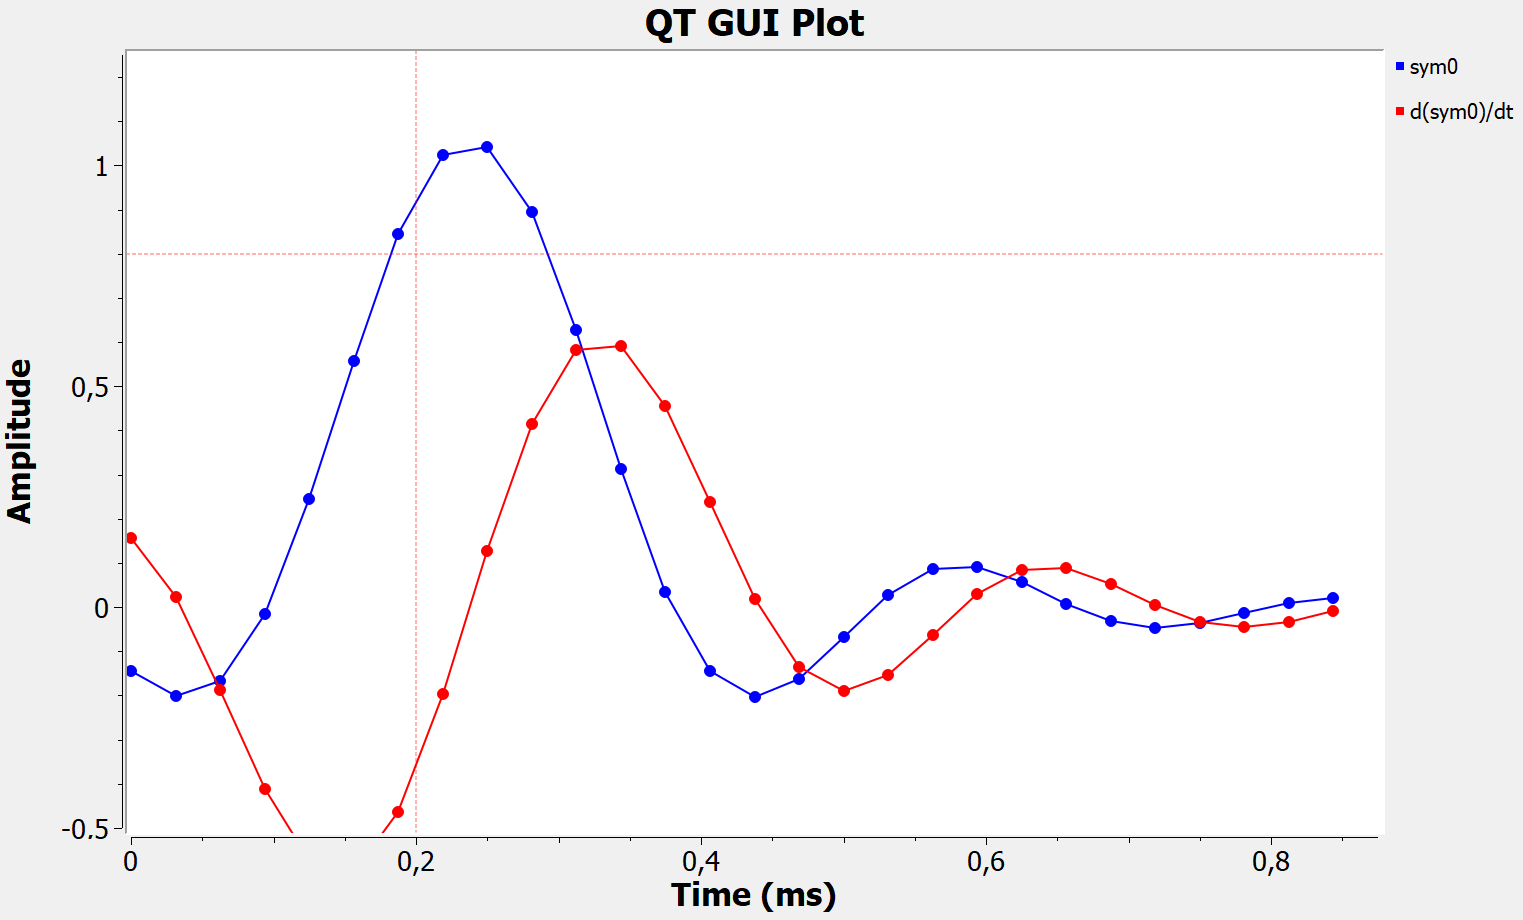
\includegraphics[width=1.0\textwidth]{lab12_fig3_6.png}
        \caption{Визуализация потокового графа}
        \label{fig:lab12_fig3_6}
\end{figure}

Но что происходит, когда у нас есть тактовое смещение? В пиковой точке дифференциальный фильтр уже не будет давать 0, как показано ниже.

\begin{figure}[H]
        \centering
        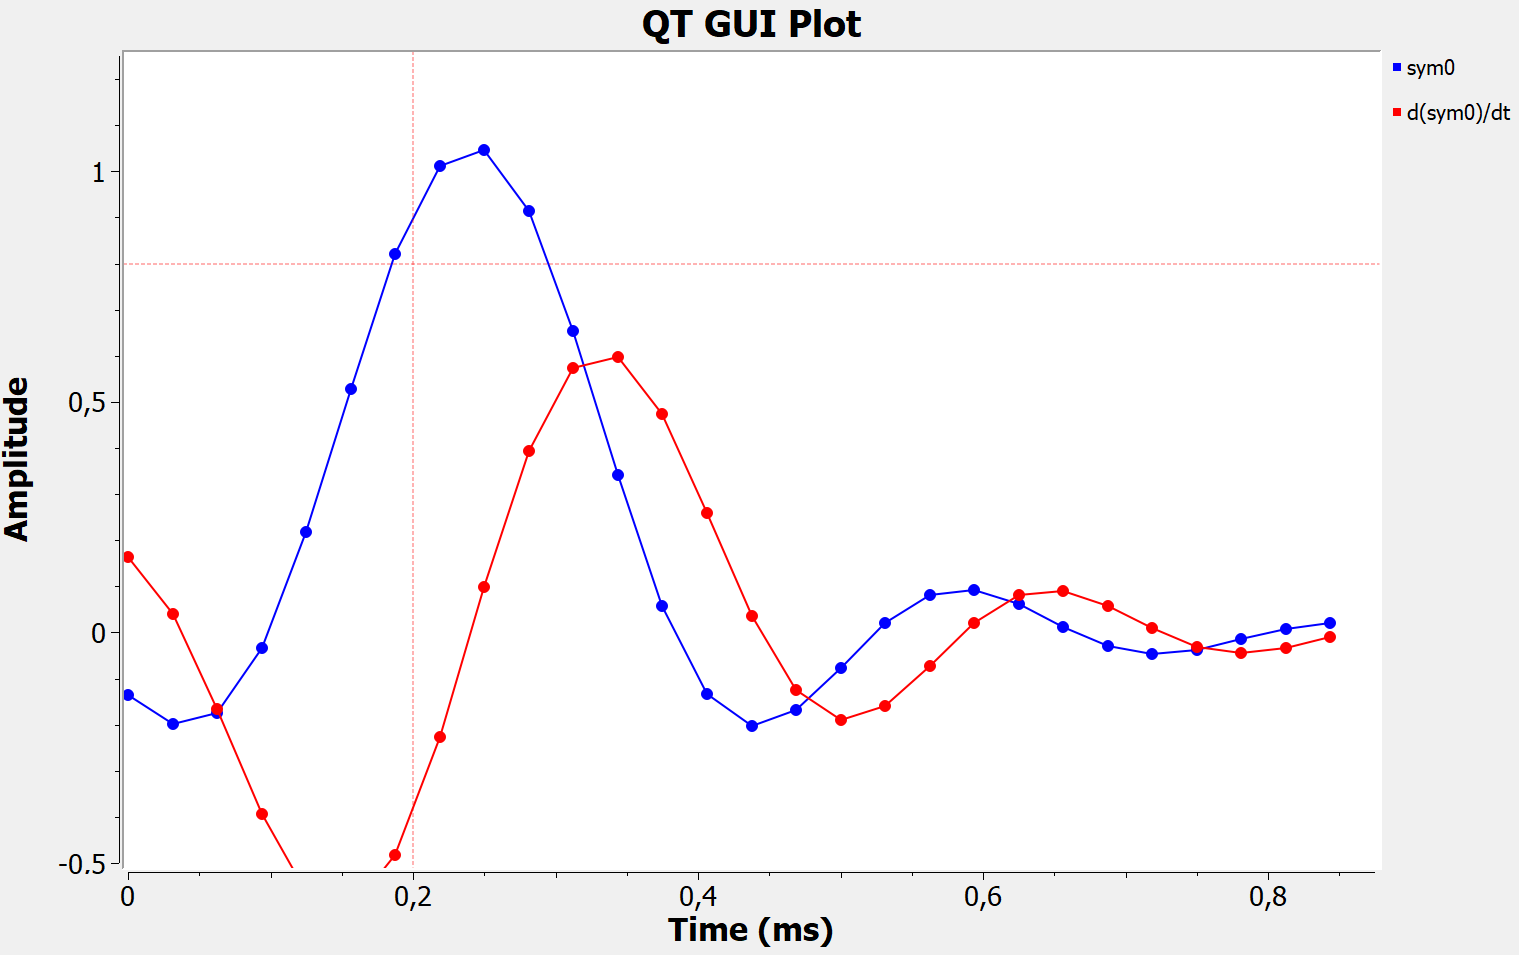
\includegraphics[width=1.0\textwidth]{lab12_fig3_7.png}
        \caption{Визуализация потокового графа со смещением}
        \label{fig:lab12_fig3_7}
\end{figure}

Вместо использования одного фильтра мы можем создать серию фильтров, где каждый с разной фазой. Если у нас достаточно фильтров на разных фазах, один из них - правильная фаза фильтра, которая даст нам желаемое значение синхронизации. Рассмотрим симуляцию, которая строит из 5 фильтров, что означает 5 различных фаз.

\begin{figure}[H]
        \centering
        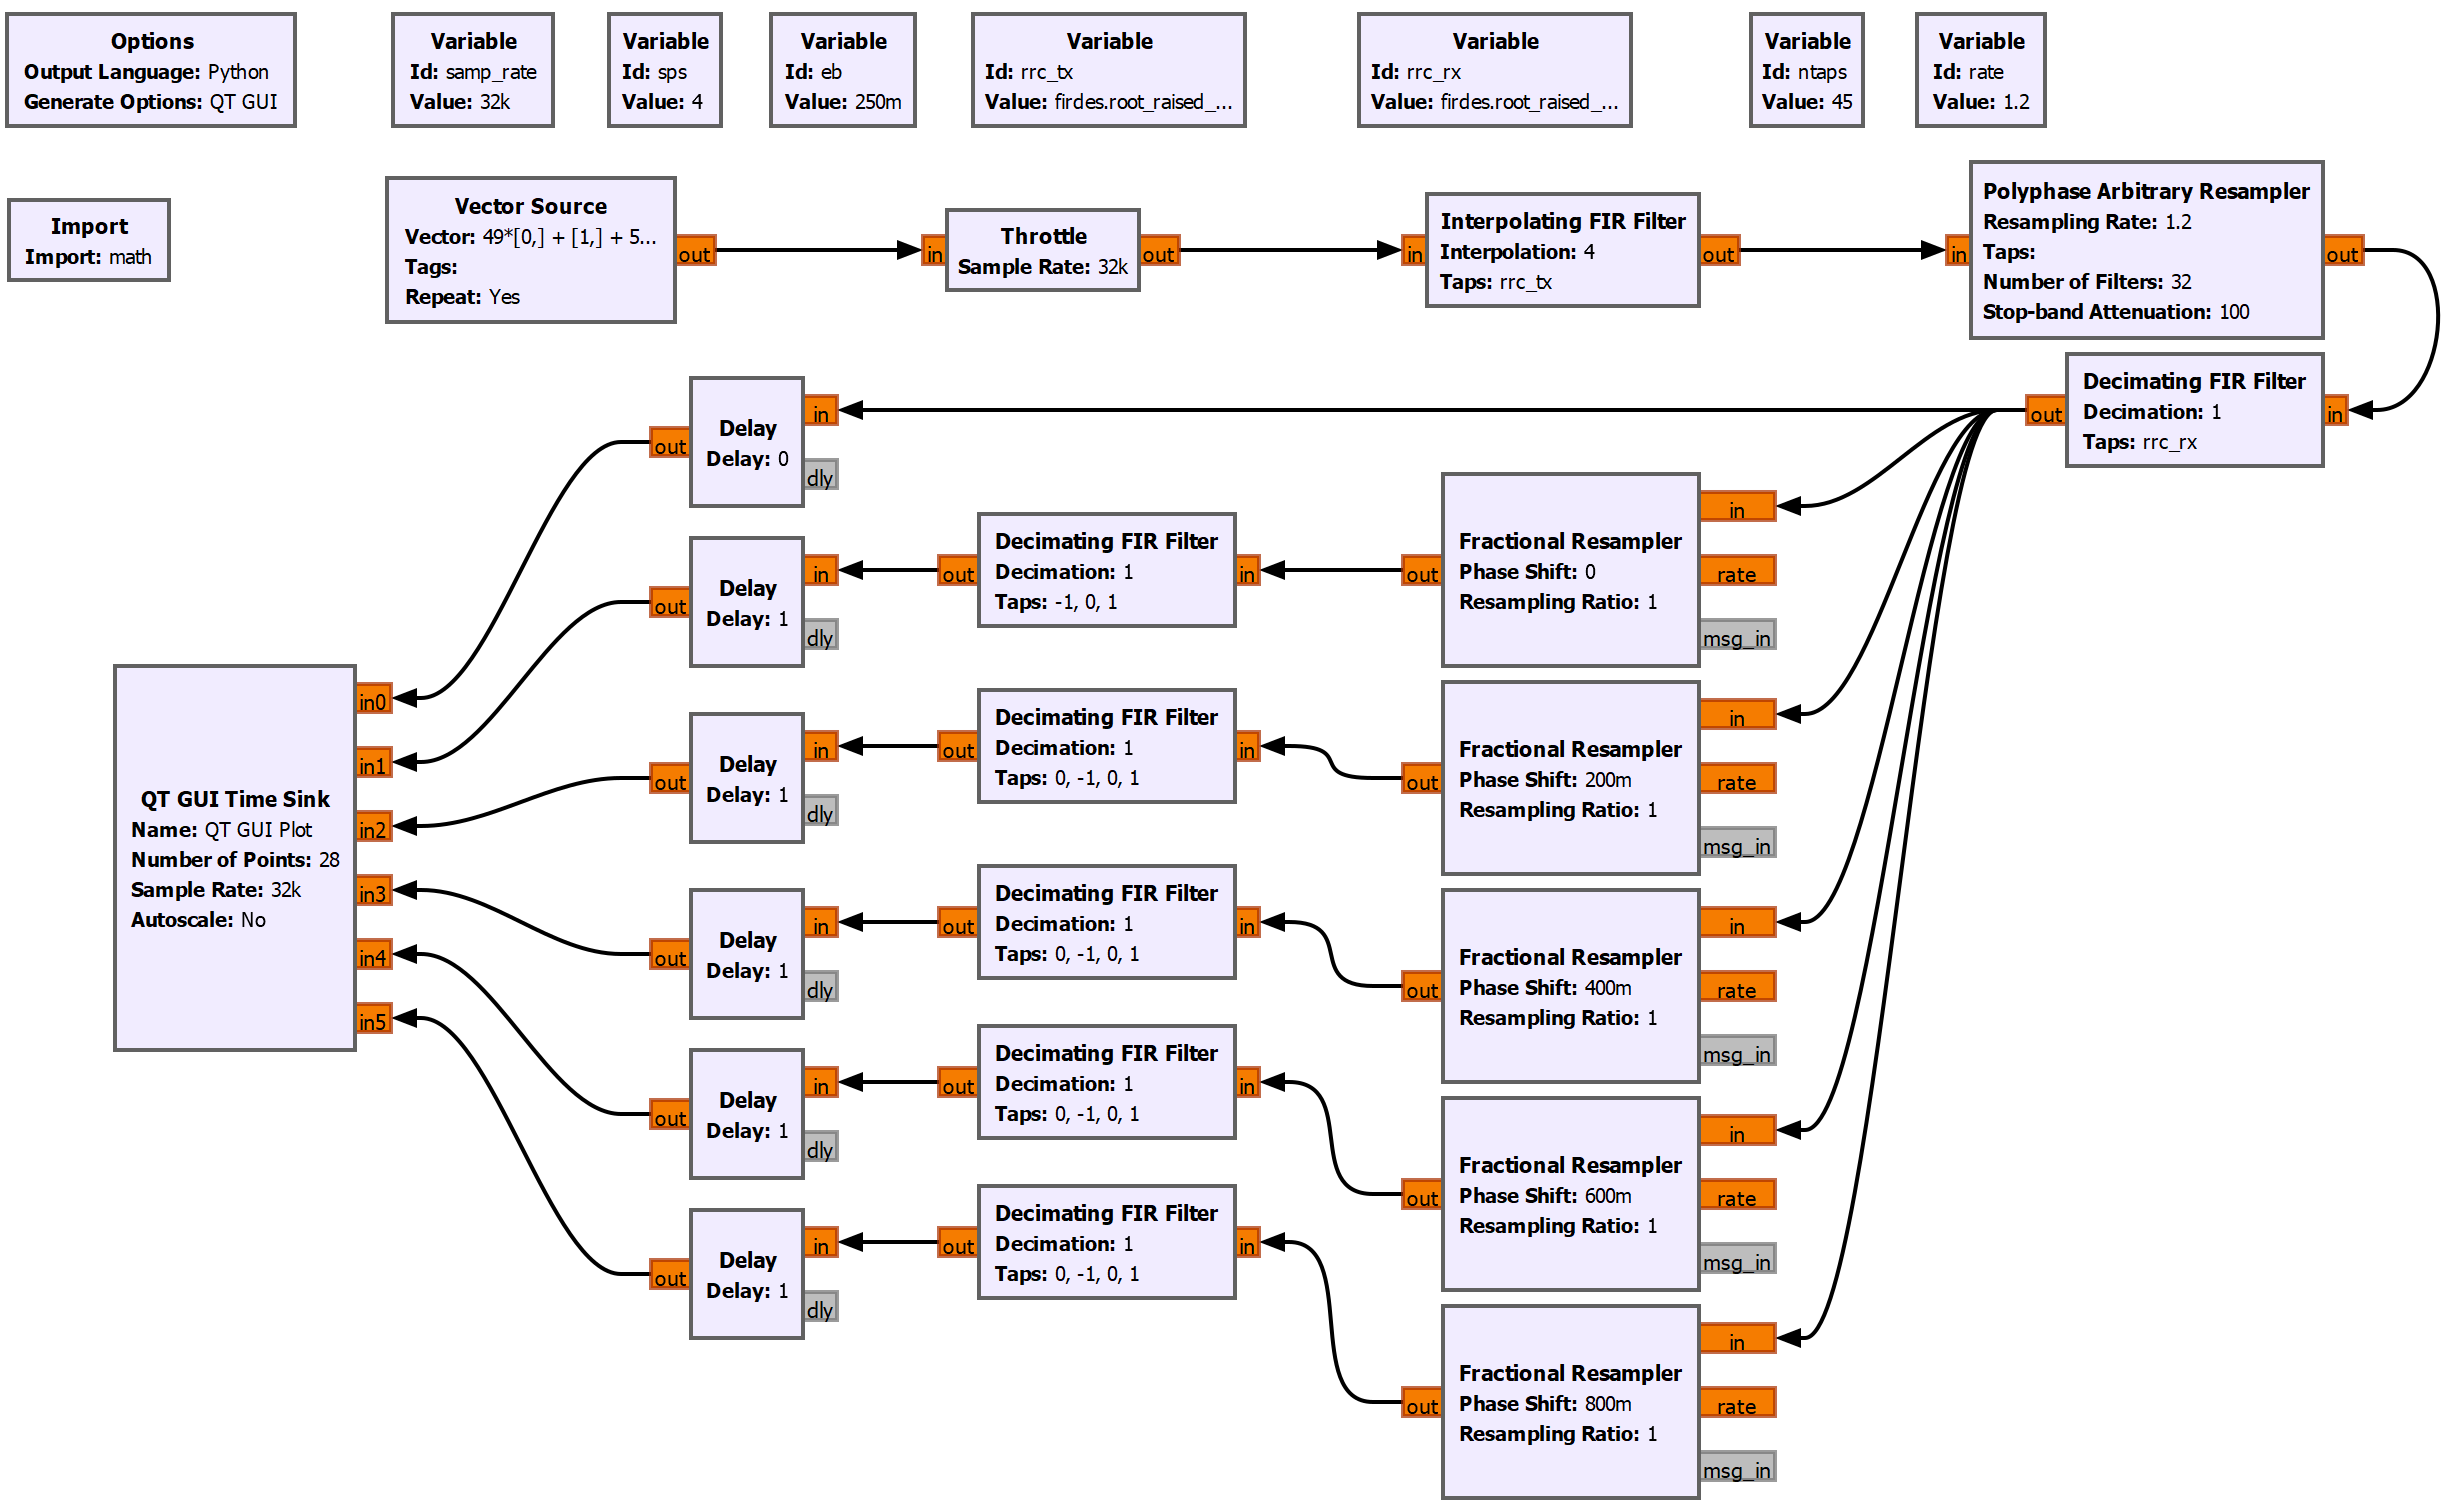
\includegraphics[width=1.0\textwidth]{lab12_fig3_8.png}
        \caption{symbol\_differential\_filter\_phases схема}
        \label{fig:lab12_fig3_8}
\end{figure}

Видно, что сигнал, помеченный как \texttt{d(sym0)/dt+phi3} в правильной точке выборки равен 0. Это говорит о том, что наша идеальная точка выборки возникает при этом сдвиге фазы. Поэтому, если мы возьмем фильтр \texttt{RRC} нашего приёмника и настроим его фазу на $3 * \frac{2}{5}\pi$, то мы сможем исправить несоответствие синхронизации и выбрать идеальную точку выборки.

\begin{figure}[H]
        \centering
        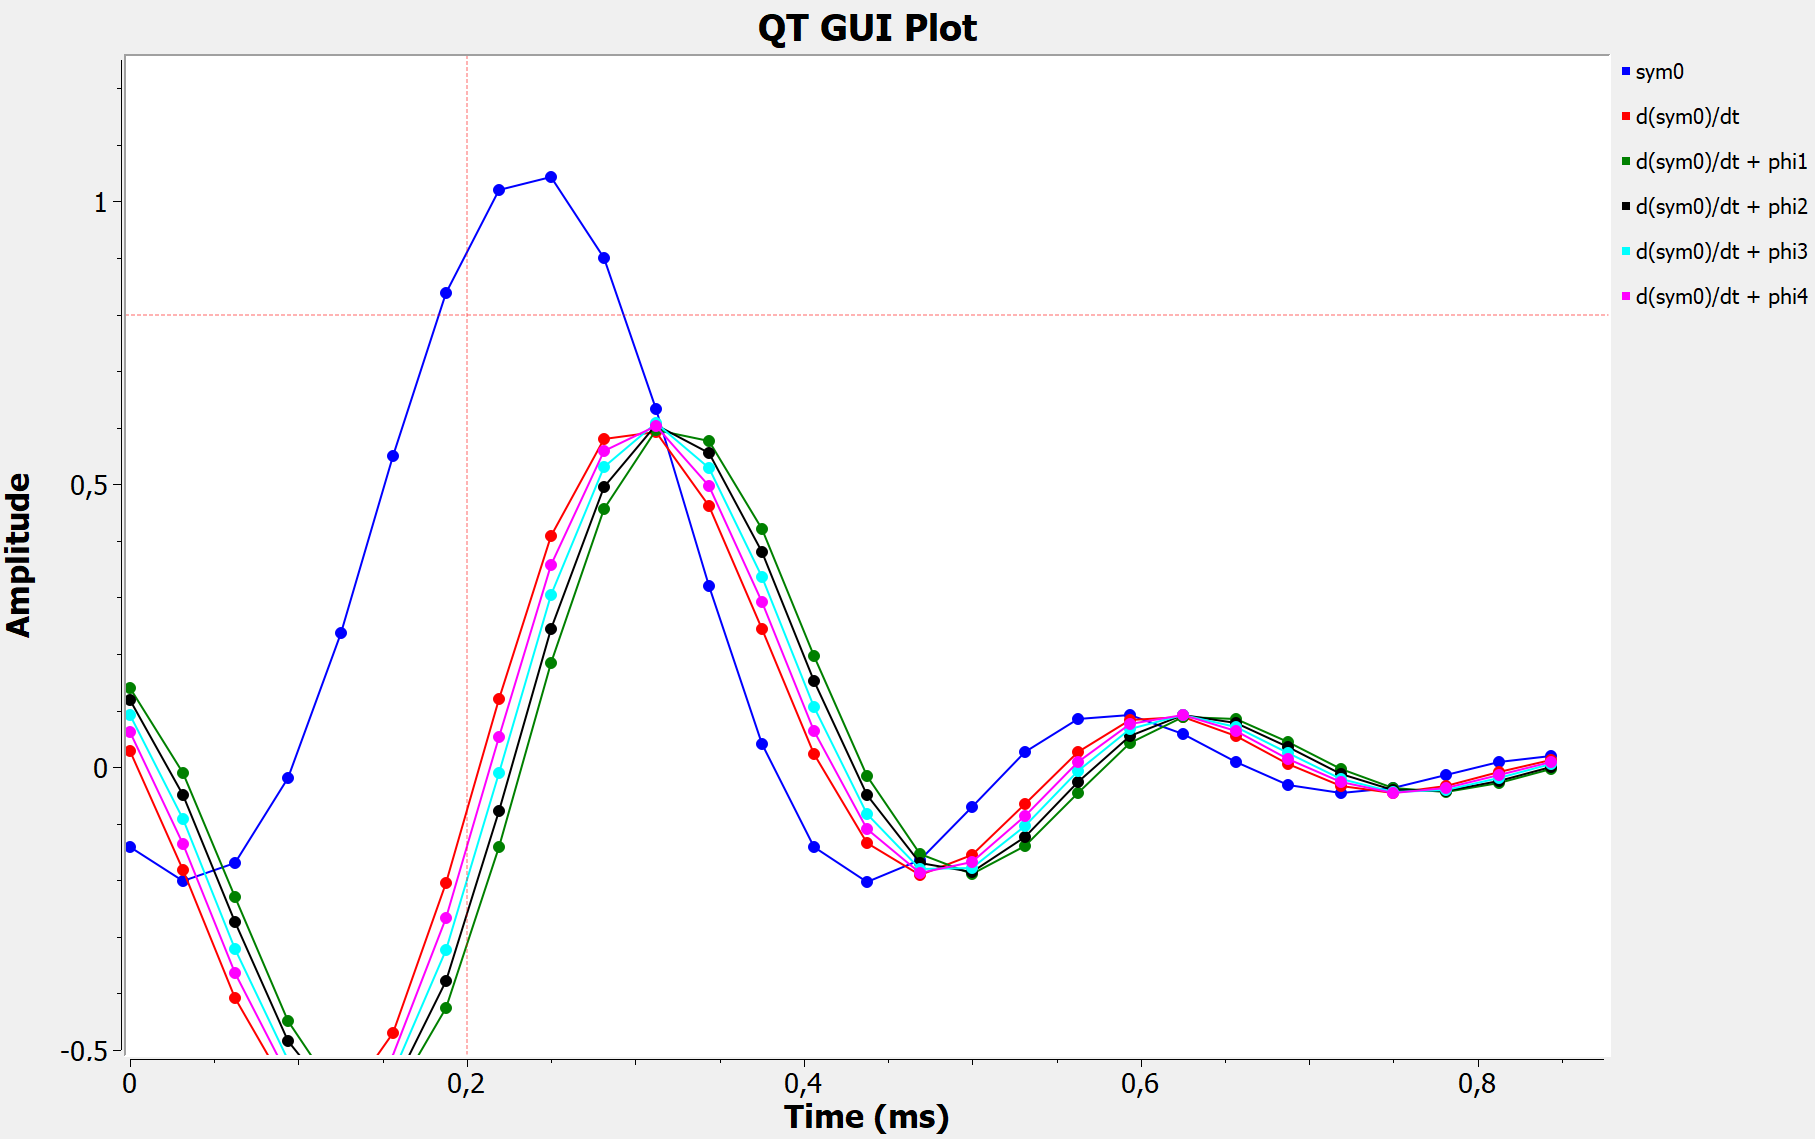
\includegraphics[width=1.0\textwidth]{lab12_fig3_9.png}
        \caption{Визуализация потокового графа с фильтрами}
        \label{fig:lab12_fig3_9}
\end{figure}

Но это лишь моделируемое приближение, в действительности выборки каждого фильтра не будут происходить в один и тот же момент времени. Чтобы действительно увидеть такое поведение, мы должны увеличить частоту дискретизации в количество раз, равное количеству фильтров.

\section{Использование блока синхронизации многофазных clock'ов в нашем приёмнике}

Теперь применим этот блок в нашей симуляции. Блок настроен с 32 фильтрами и полосой пропускания петли $\frac{2}{100}\pi$.

\begin{figure}[H]
        \centering
        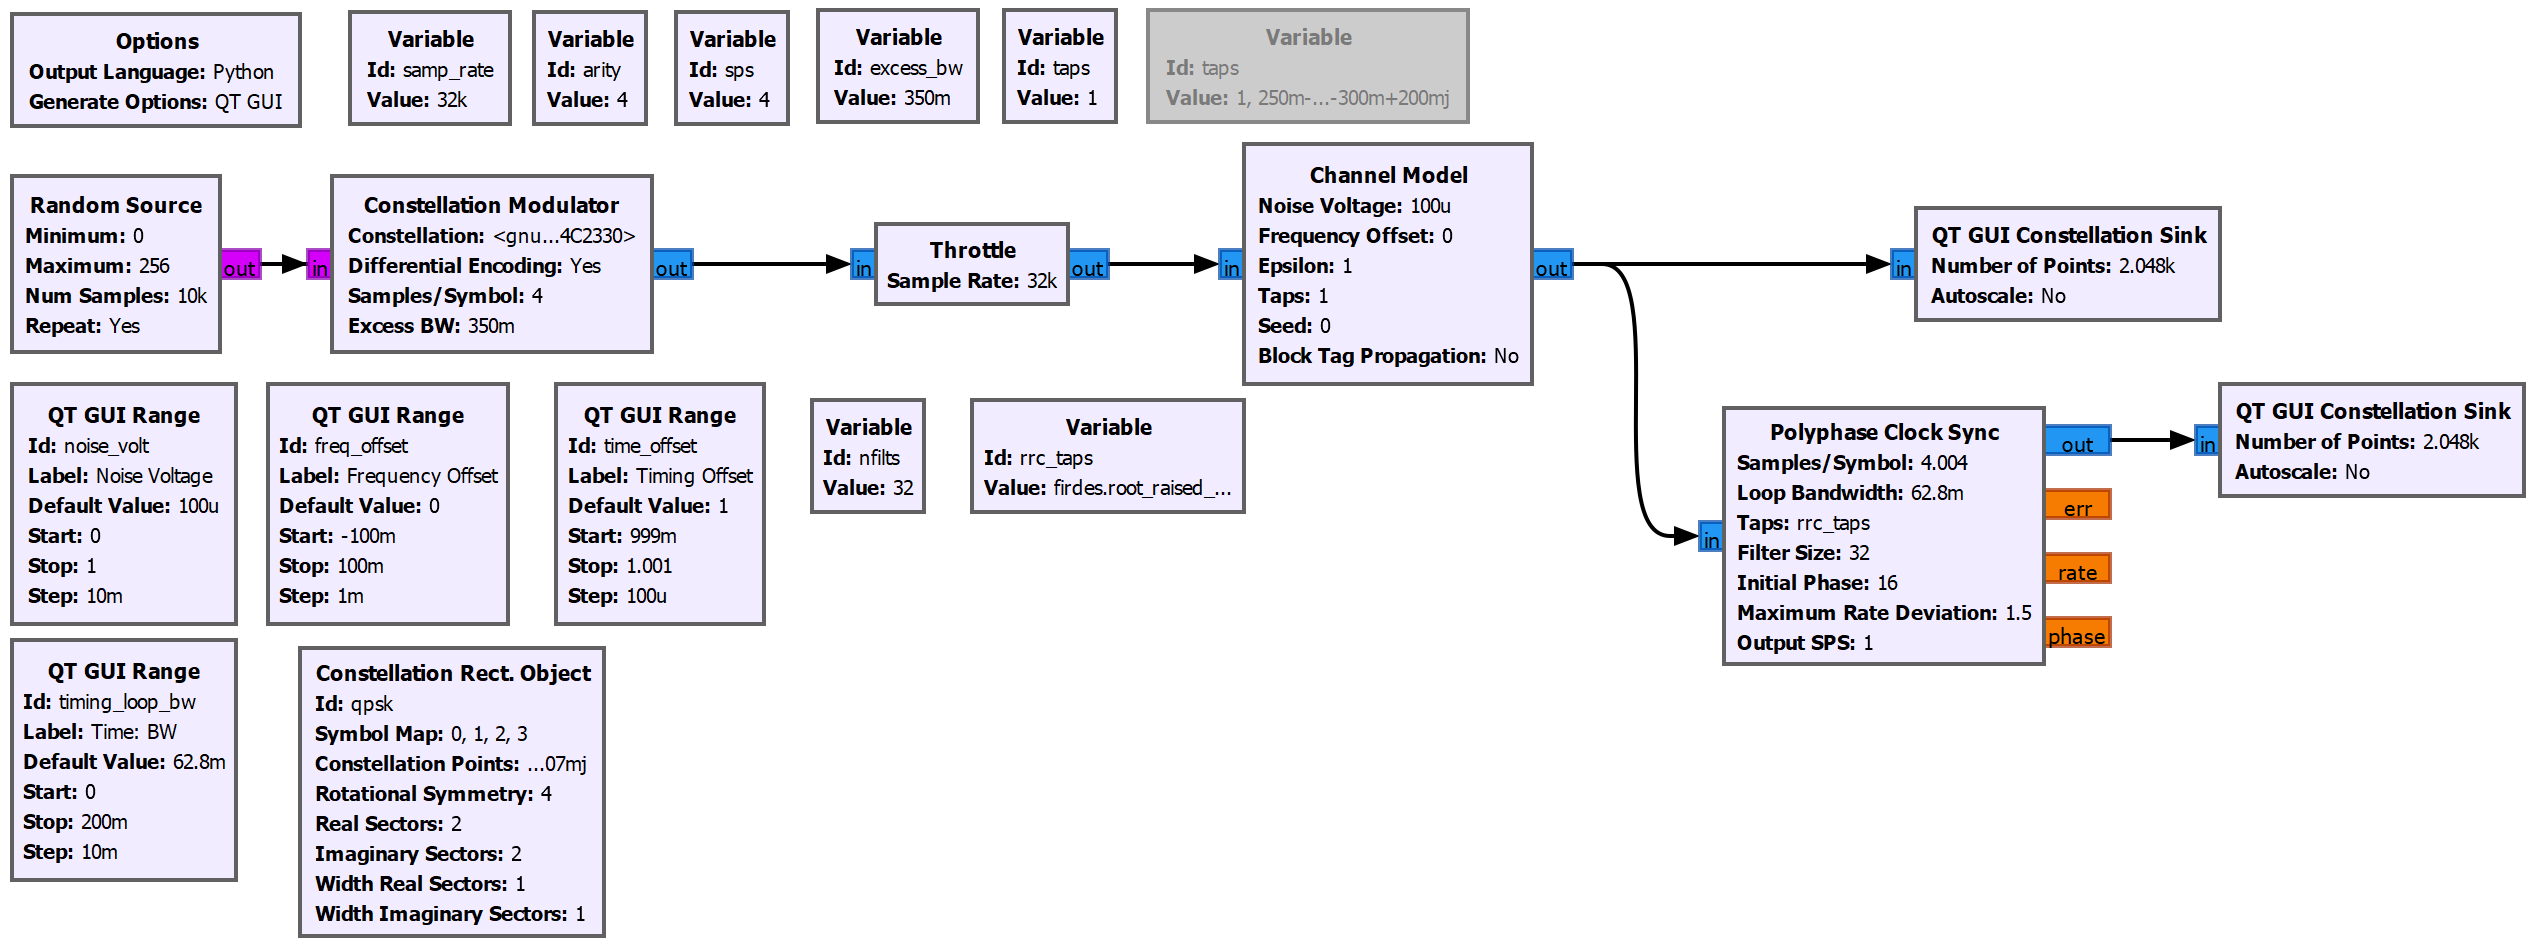
\includegraphics[width=1.0\textwidth]{lab12_fig3_10.png}
        \caption{mpsk\_stage3 схема}
        \label{fig:lab12_fig3_10}
\end{figure}

\begin{figure}[H]
        \centering
        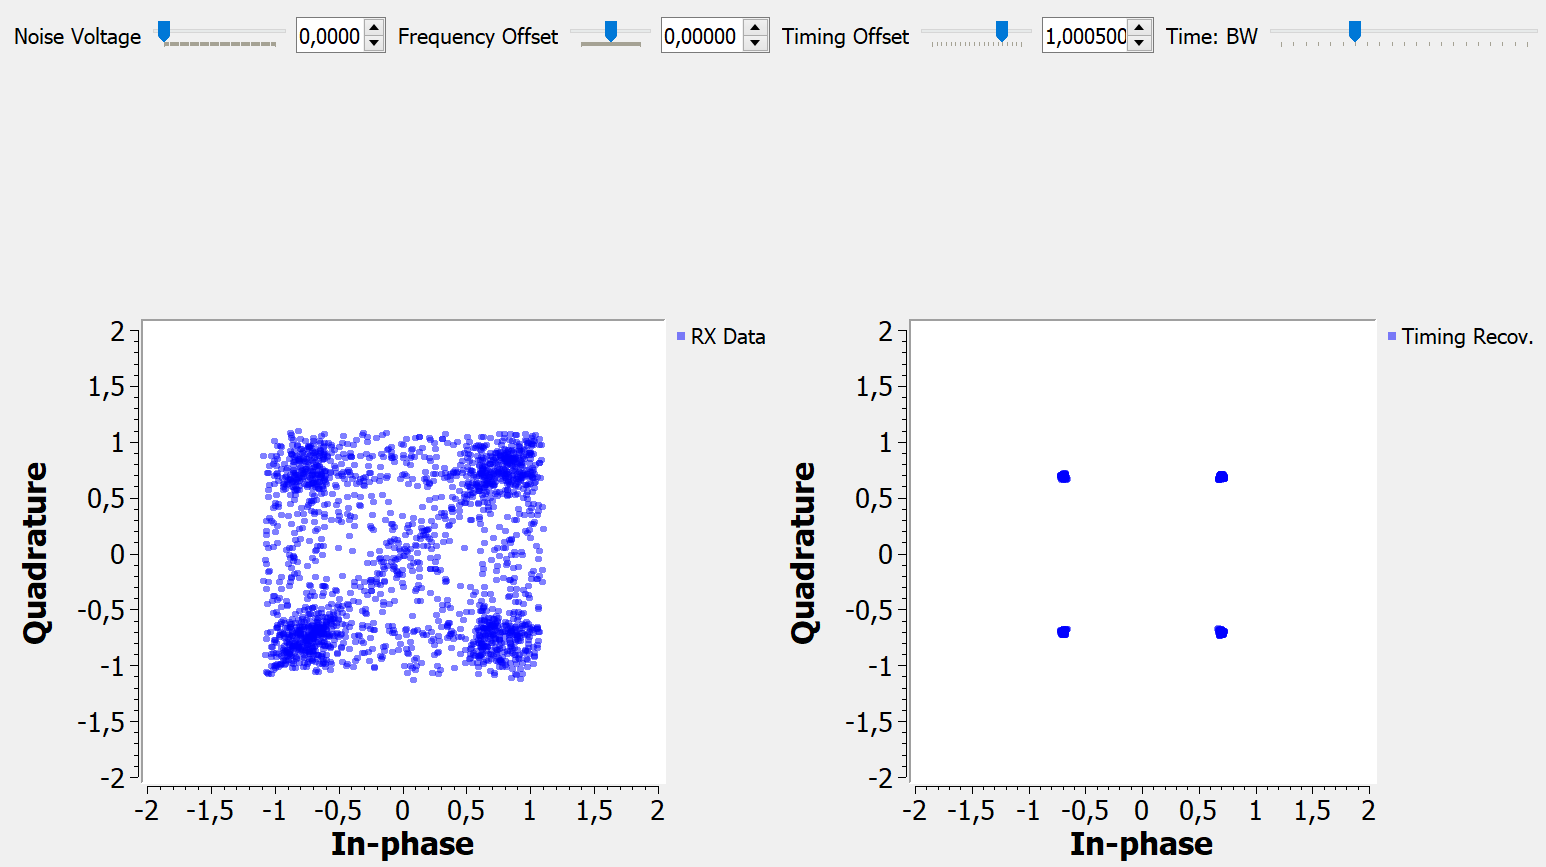
\includegraphics[width=1.0\textwidth]{lab12_fig3_11.png}
        \caption{Визуализация графа}
        \label{fig:lab12_fig3_11}
\end{figure}

На графике слева - сигнал до синхронизации, справа - после. Он всё ещё немного зашумлён из-за \texttt{ISI}, но этот шум быстро поглощается другим шумом при установке \texttt{Noise Voltage} для каналов отличным от нуля:

\begin{figure}[H]
        \centering
        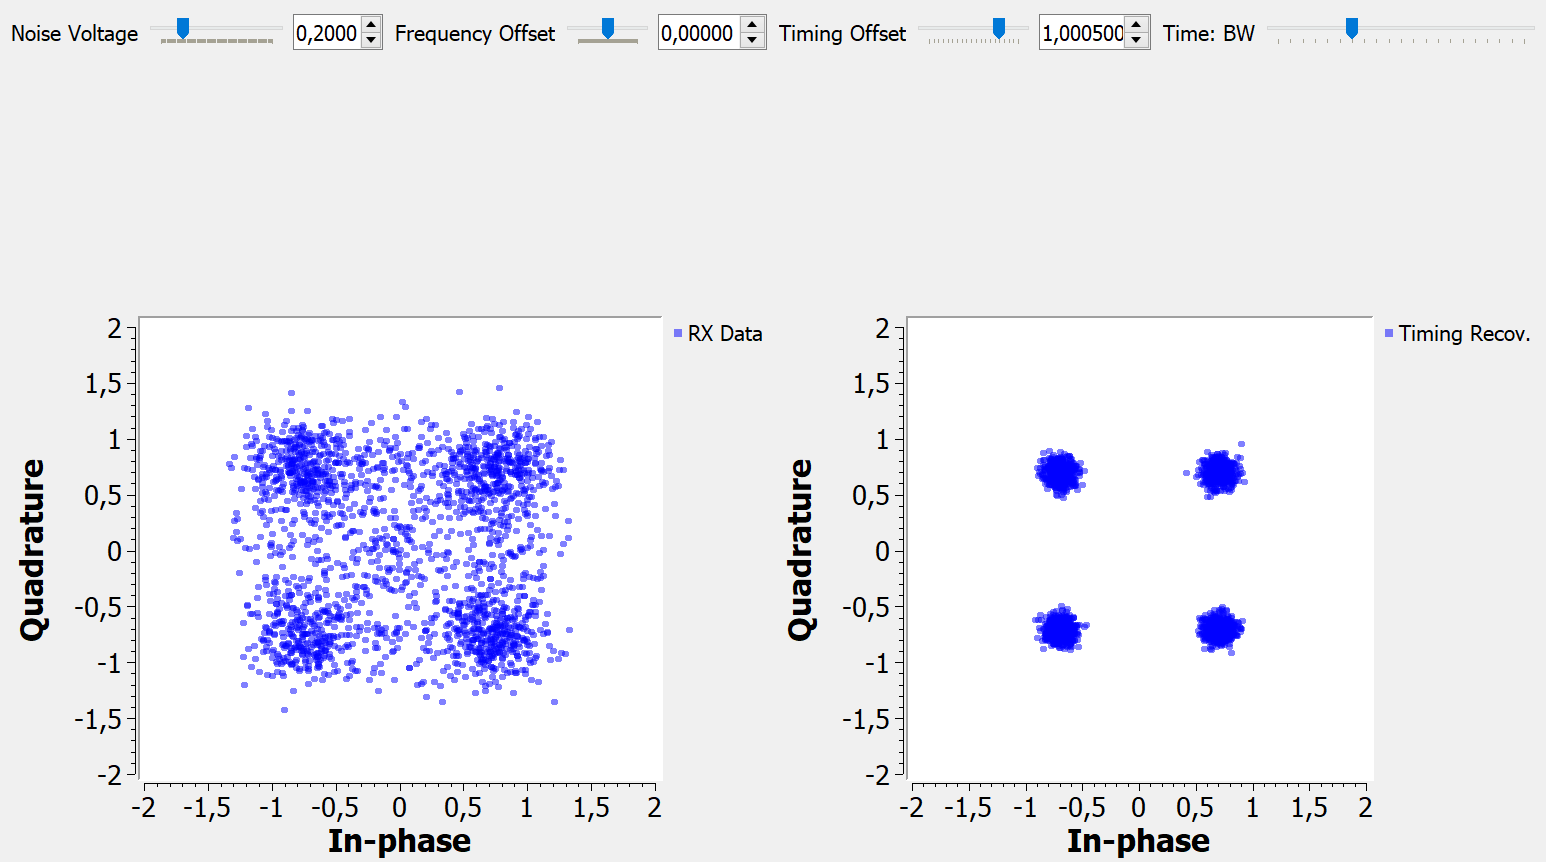
\includegraphics[width=1.0\textwidth]{lab12_fig3_12.png}
        \caption{Удаление шума}
        \label{fig:lab12_fig3_12}
\end{figure}

Если добавить смещение частоты, то созвездие станет окружностью. Созвездие всё ещё будет находится на единичной окружности, что означает, что тактовая синхронизация сохраняется, но блок не позволяет нам корректировать смещение частоты.

\begin{figure}[H]
        \centering
        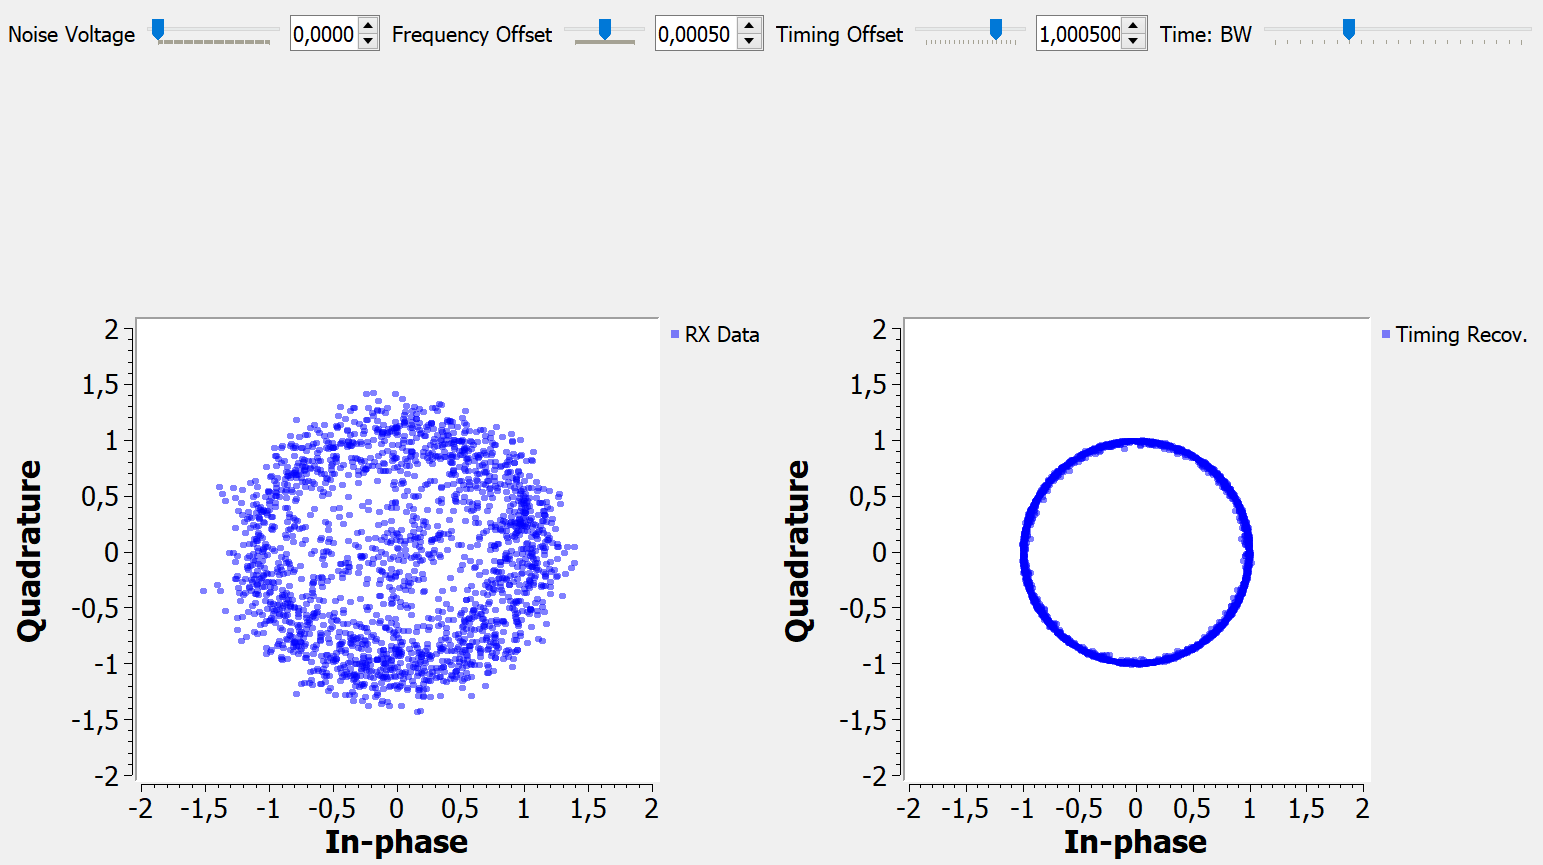
\includegraphics[width=1.0\textwidth]{lab12_fig3_13.png}
        \caption{Добавление смещения частоты}
        \label{fig:lab12_fig3_13}
\end{figure}

\chapter{Многолучевое распространение}

Воздействие комбинации сигналов на приёмник при многолучевом распространении - искажение сигнала. Если разница во времени между отражениями достаточно мала по сравнению с шириной символа, искажение может быть внутри символа - внутри-символьная интерференция. Если время отражения превышает время символа, отражение от одного символа будет влиять на следующие сигналы - ещё одна причина межсимвольной интерференции.

Чтобы исправить это поведение, мы можем использовать механизм, очень похожий на стереоэквалайзер. С помощью стереофонического эквалайзера мы можем изменить усиление определенных частот, чтобы либо подавить, либо усилить эти сигналы, наиболее распространенными из которых являются низкие и высокие частоты.

К сожалению, по каким-то причинам библиотеки scipy не было в файлах gnuradio, поэтому пришлось добавить её вручную.

\begin{figure}[H]
        \centering
        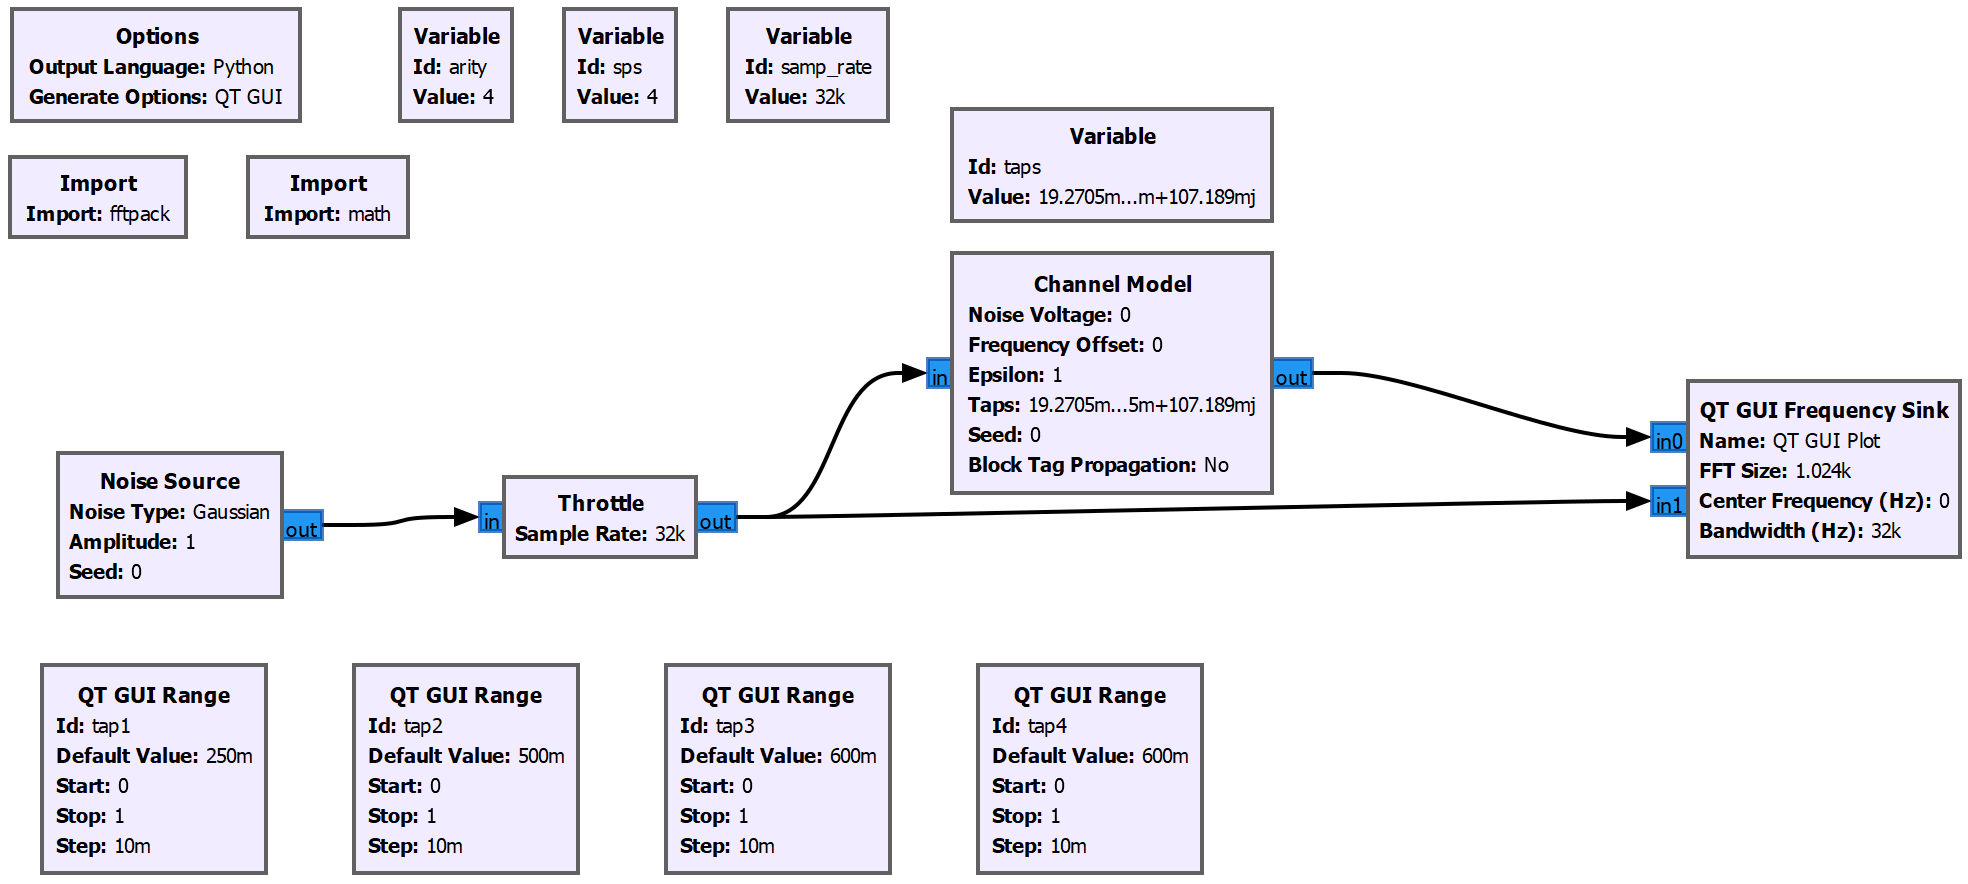
\includegraphics[width=1.0\textwidth]{lab12_fig4_1.png}
        \caption{multipath\_sim схема}
        \label{fig:lab12_fig4_1}
\end{figure}

Это моделирование настраивает модель канала, чтобы предоставить каналу пять элементов управления эквалайзером, четыре из которых мы можем изменить. Хотя в этом примере мы явно контролируем частотную область, на самом деле мы играем с возможностью создать эквалайзер, который может корректировать или регулировать частотную характеристику принятого сигнала. В конечном итоге цель показана на рисунке ниже, где многолучевой канал создает некоторые искажения в сигнале, как показано в частотной области. Задача эквалайзера - инвертировать этот канал.

\begin{figure}[H]
        \centering
        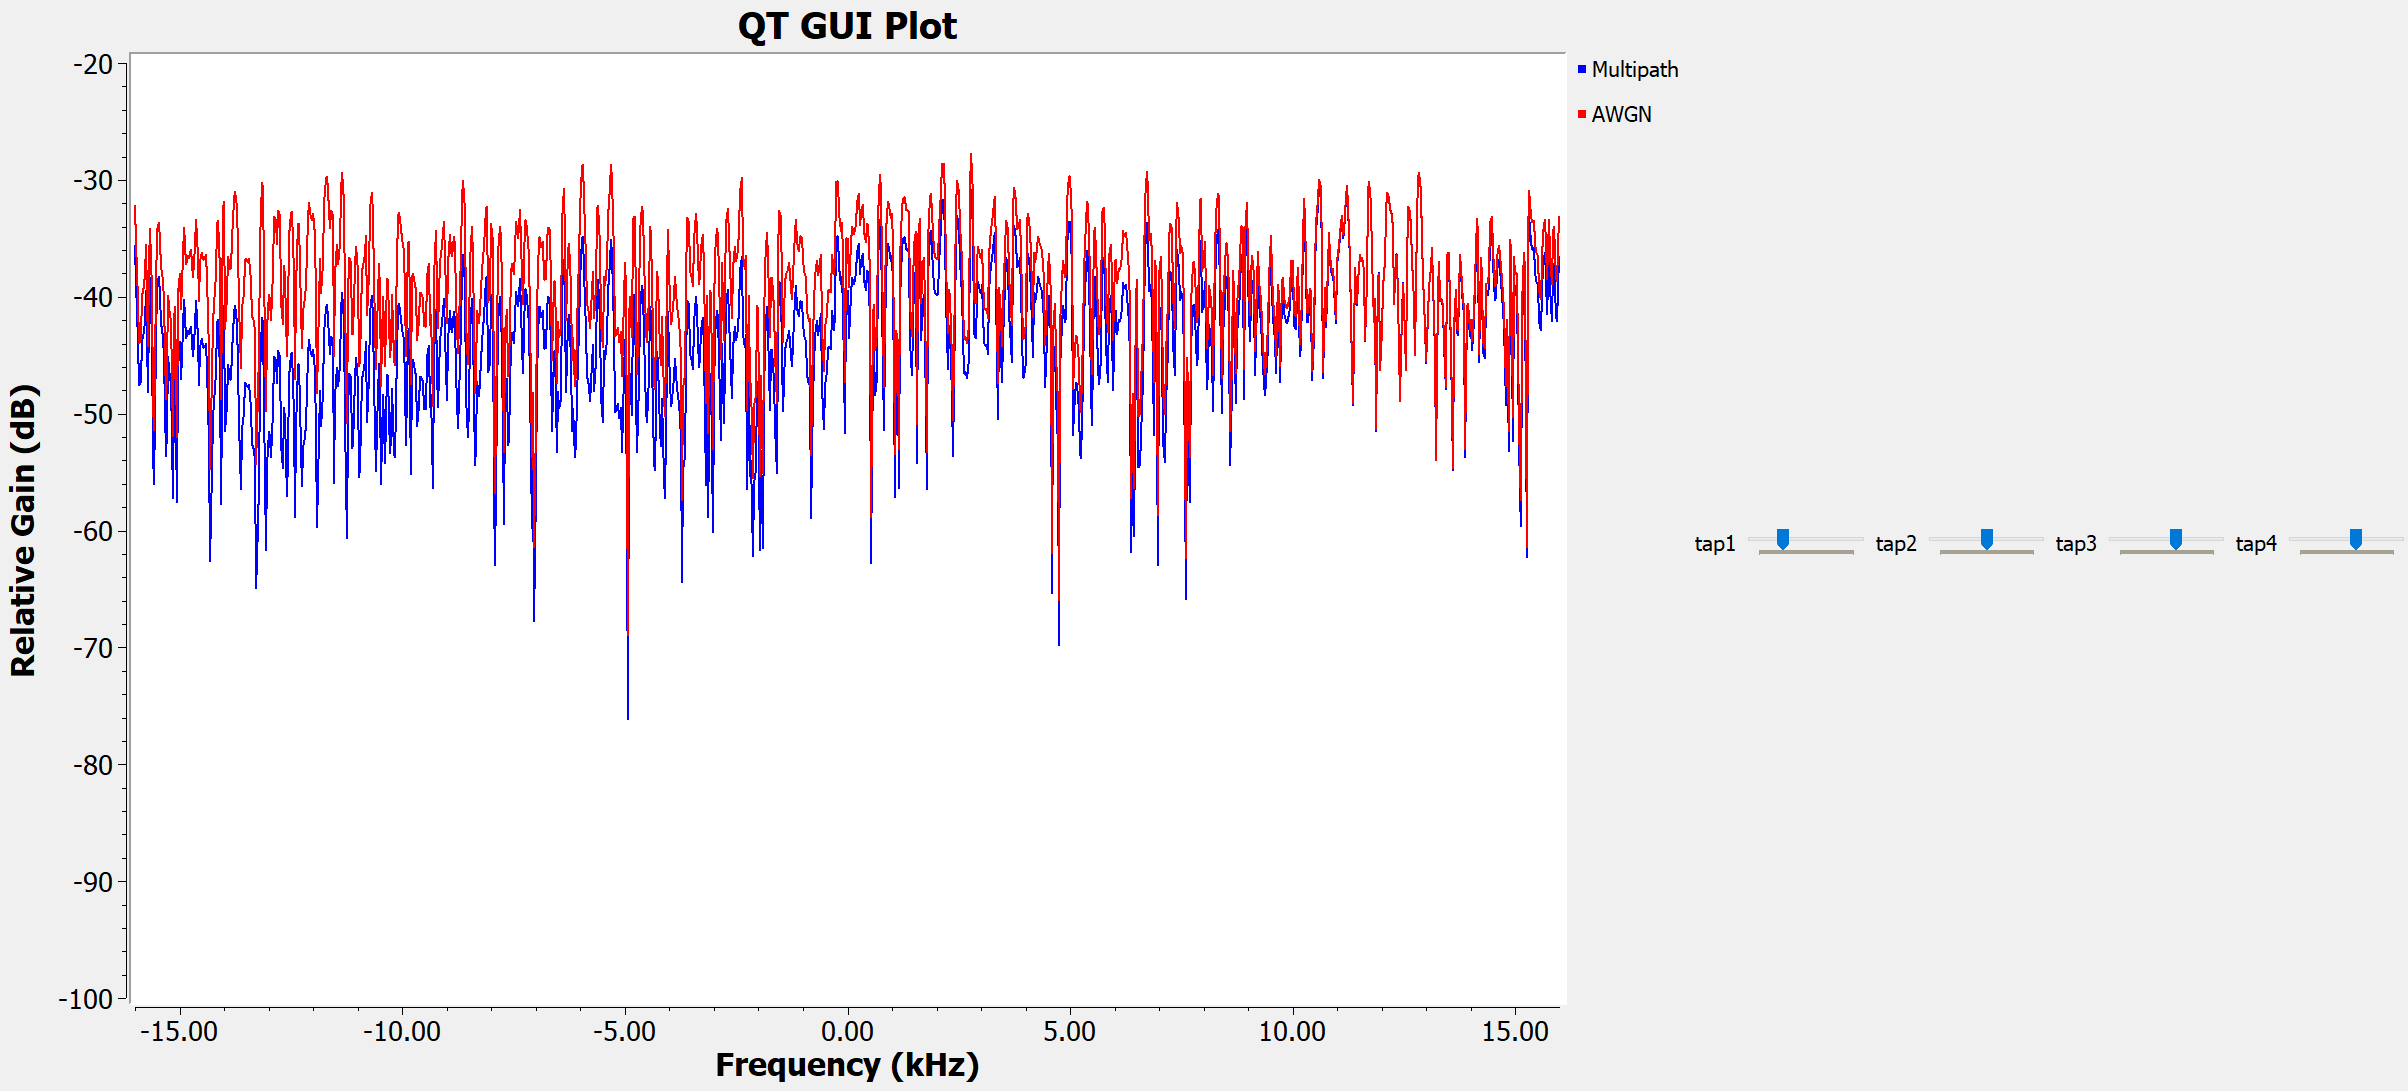
\includegraphics[width=1.0\textwidth]{lab12_fig4_2.png}
        \caption{Визуализация графа}
        \label{fig:lab12_fig4_2}
\end{figure}

\chapter{Эквалайзеры}

GNU Radio поставляется с двумя легко используемыми эквалайзерами, \texttt{CMA} и \texttt{DD LMS}. Мы сначала будем использовать \texttt{CMA (Constant Modulus Algorithm)}, а затем \texttt{DD LMS (Decision-Directed Least Mean Squared)}. CMA или алгоритм постоянного модуля - это слепой эквалайзер, но он работает только с сигналами с постоянной амплитудой или модулем. В примере ниже мы используем алгоритм CMA с 11 taps.

\begin{figure}[H]
        \centering
        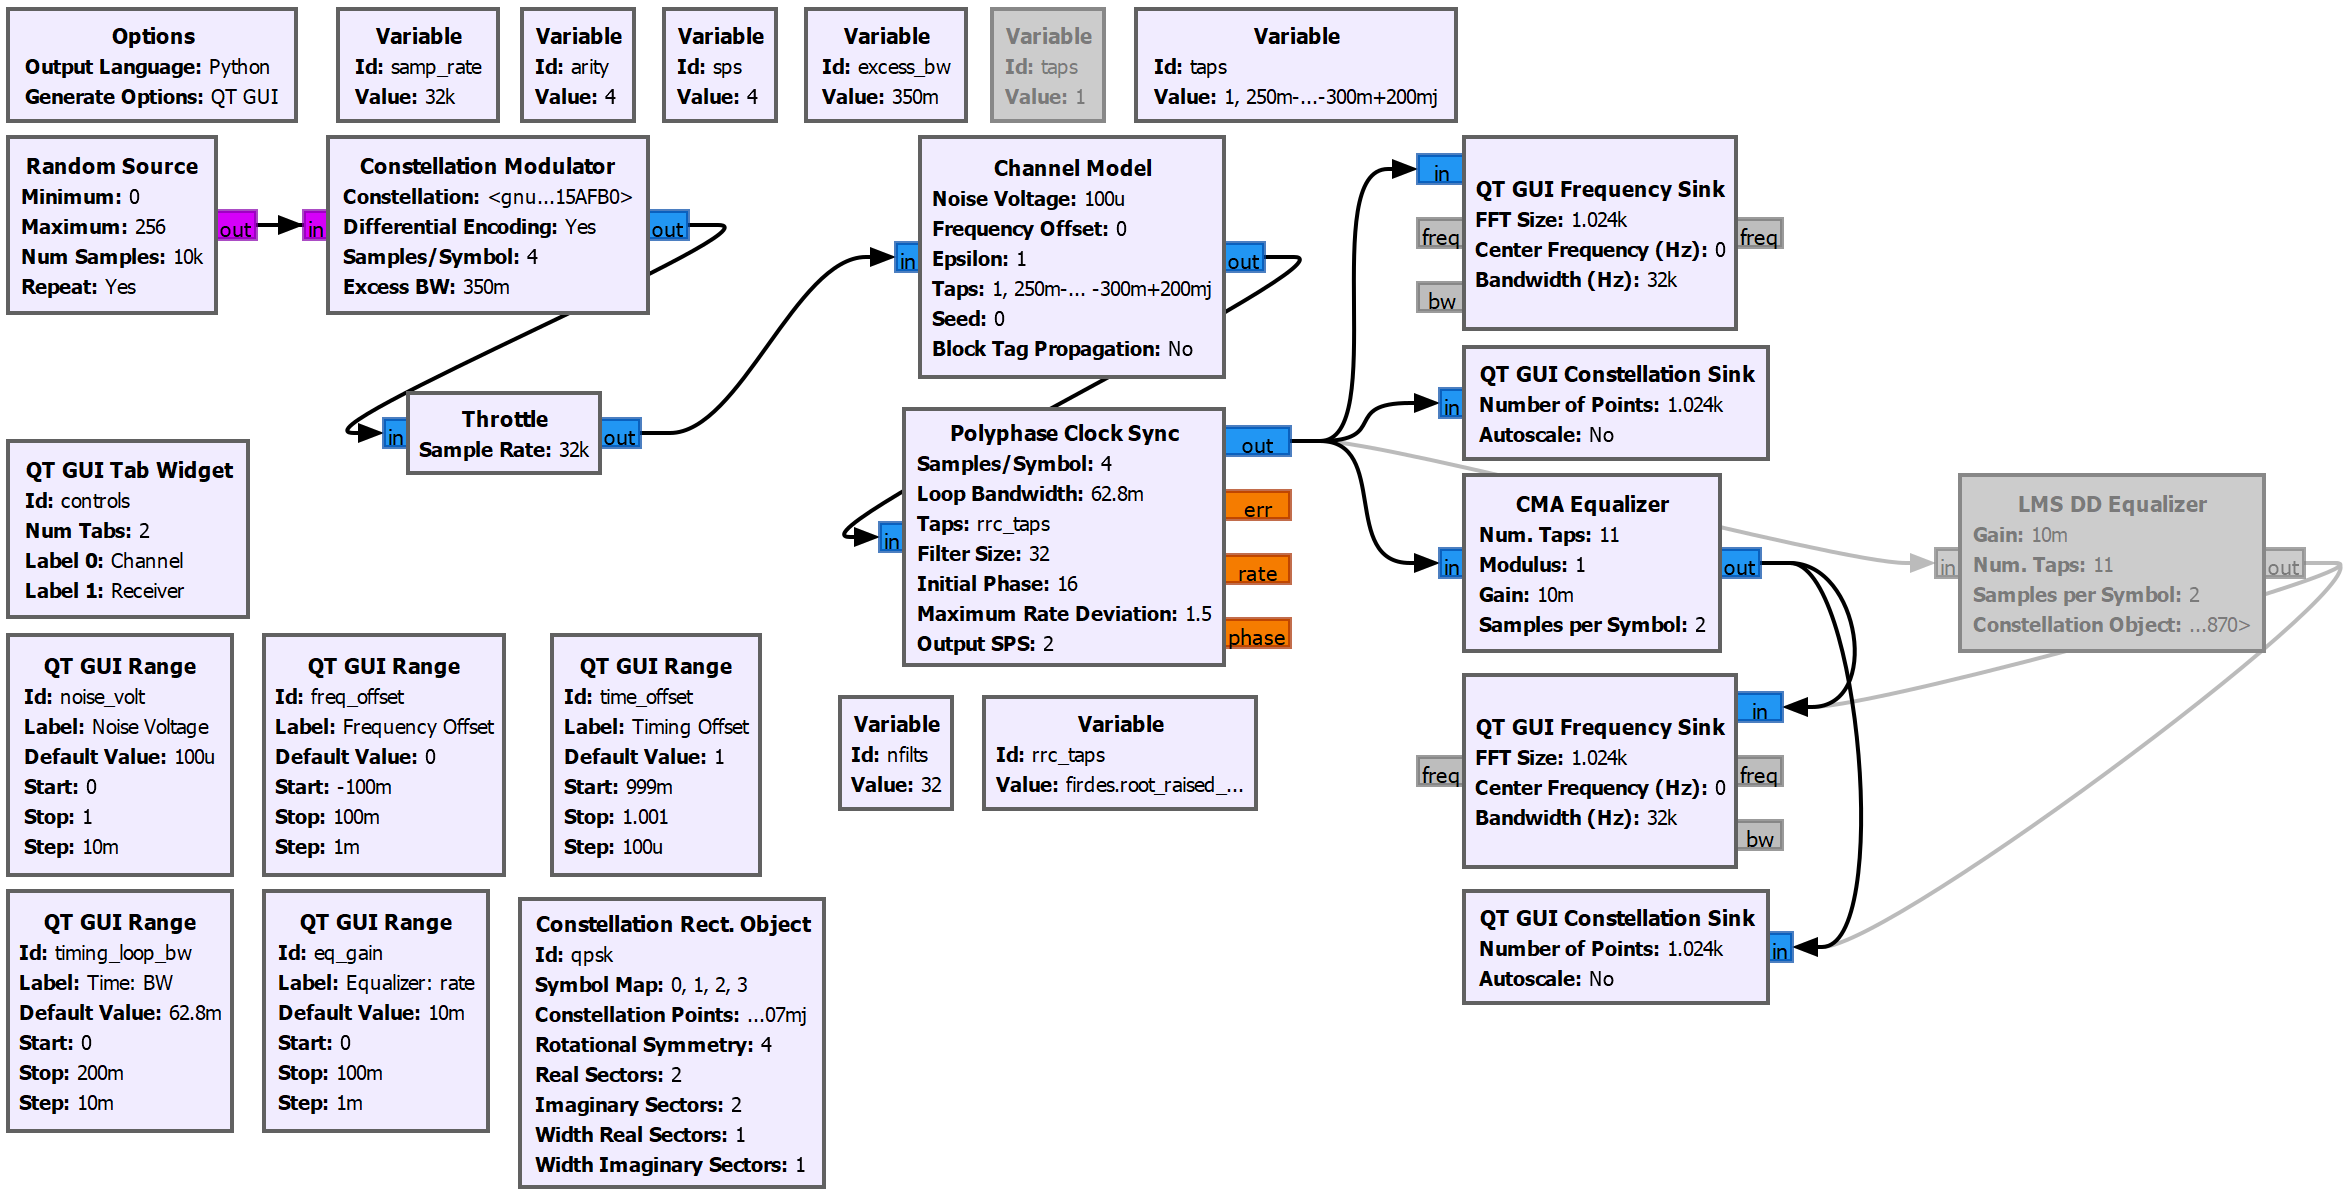
\includegraphics[width=1.0\textwidth]{lab12_fig5_1.png}
        \caption{mpsk\_stage4 граф с \texttt{CMA}}
        \label{fig:lab12_fig5_1}
\end{figure}

Мы можем наблюдать сходимость алгоритма \texttt{CMA}. Перед эквалайзером у нас очень некрасивый сигнал даже без шумов. Эквалайзер прекрасно понимает, как инвертировать и отменить этот канал, чтобы у нас снова был хороший, чистый сигнал. Мы также можем видеть сам канал и то, как он красиво выравнивается после эквалайзера.

\begin{figure}[H]
        \centering
        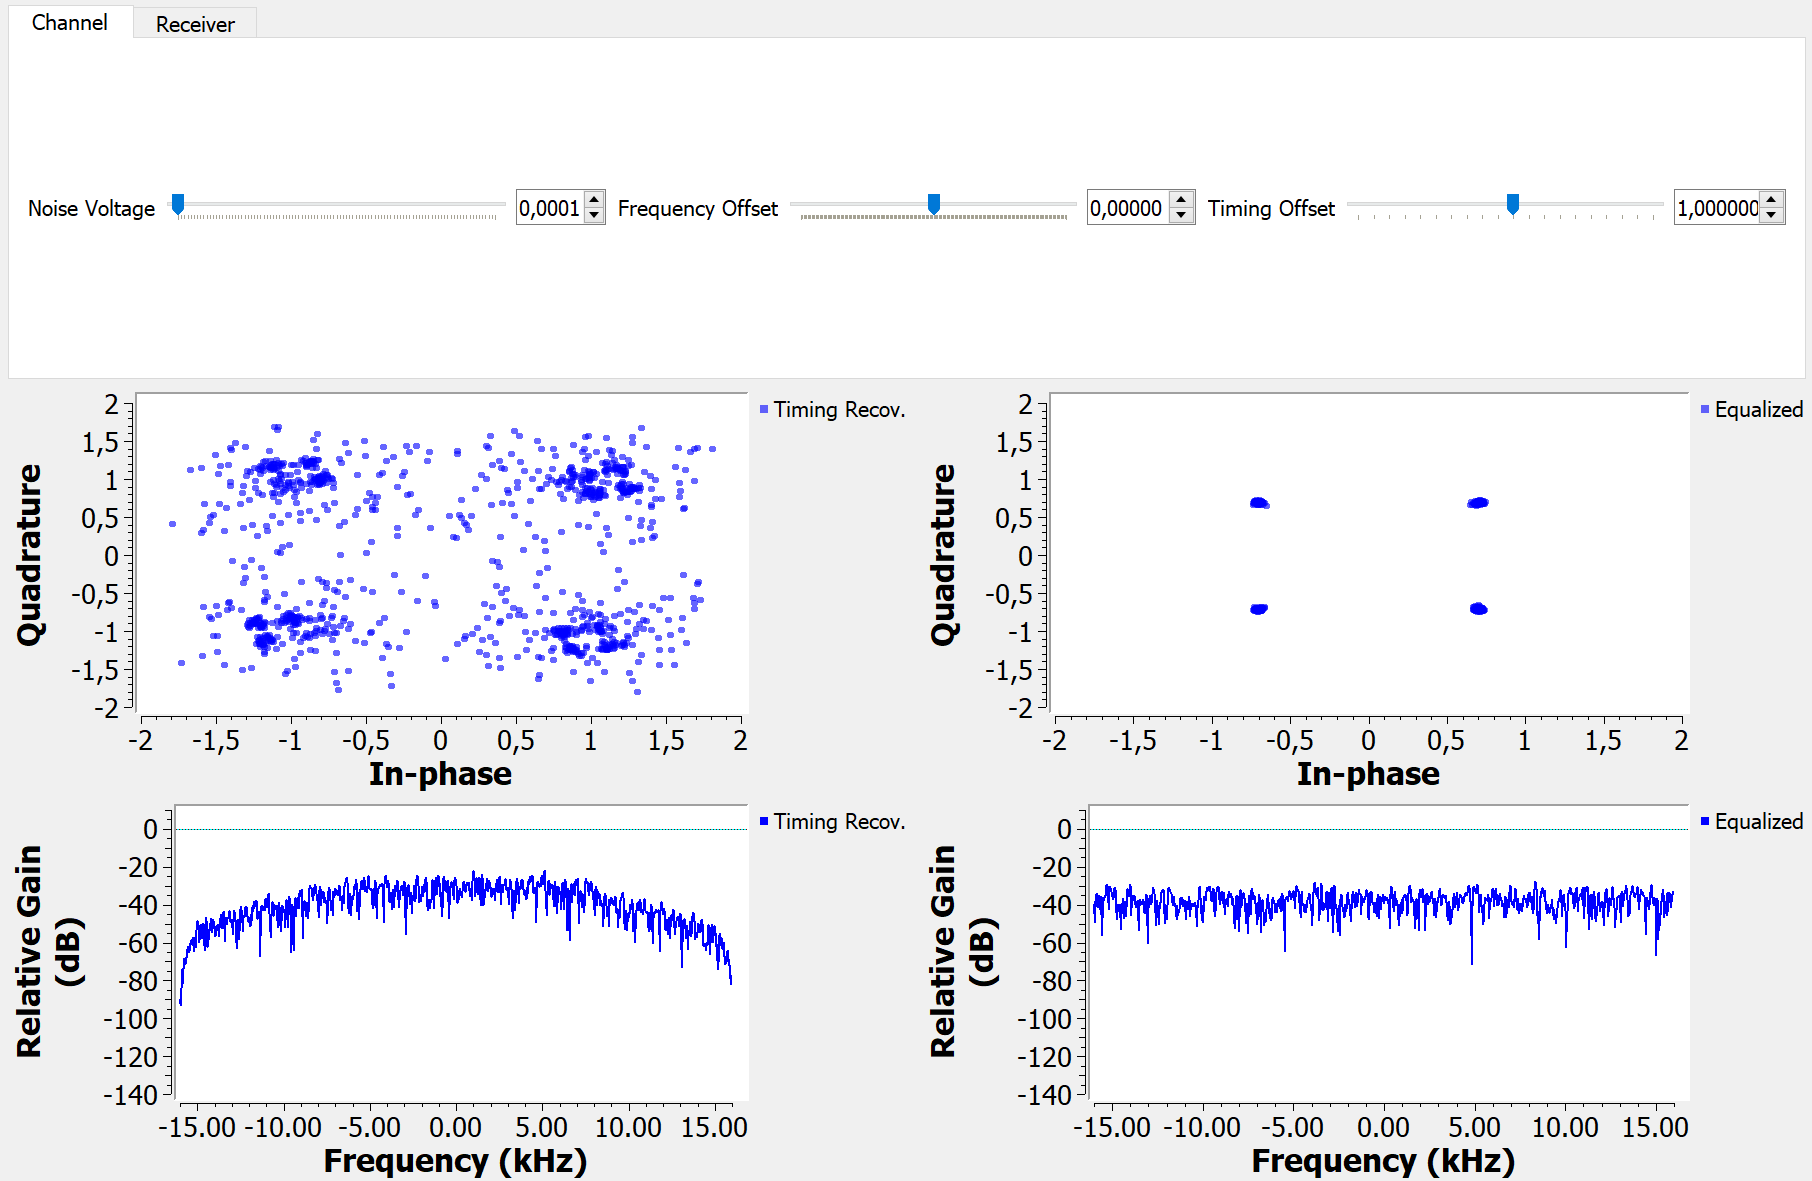
\includegraphics[width=1.0\textwidth]{lab12_fig5_2.png}
        \caption{Визуализация данных графа}
        \label{fig:lab12_fig5_2}
\end{figure}

Теперь рассмотрим \texttt{DD LMS}. \texttt{CMA} и \texttt{DD LMS} довольно похожи в плане параметров, за исключением одной важной особенности. \texttt{DD LMS}, в отличие от \texttt{CMA} – не слепой эквалайзер, он требует информации о принимаемом сигнале. Ему необходимо знать точки созвездия. Этот эквалайзер отлично подходит для сигналов, которые не соответствуют требованию постоянного модуля алгоритма \texttt{CMA}. С другой стороны, если \texttt{SNR} достаточно плох, принимаемые решения будут неправильными, что может ухудшить производительность приемника. Кроме того, \texttt{DD LMS} более сложен в вычислительном отношении. Для \texttt{DD LMS} рассматривать графики не будем, так как результат на них максимально близок с теми, что мы рассмотрели ранее.

\begin{figure}[H]
        \centering
        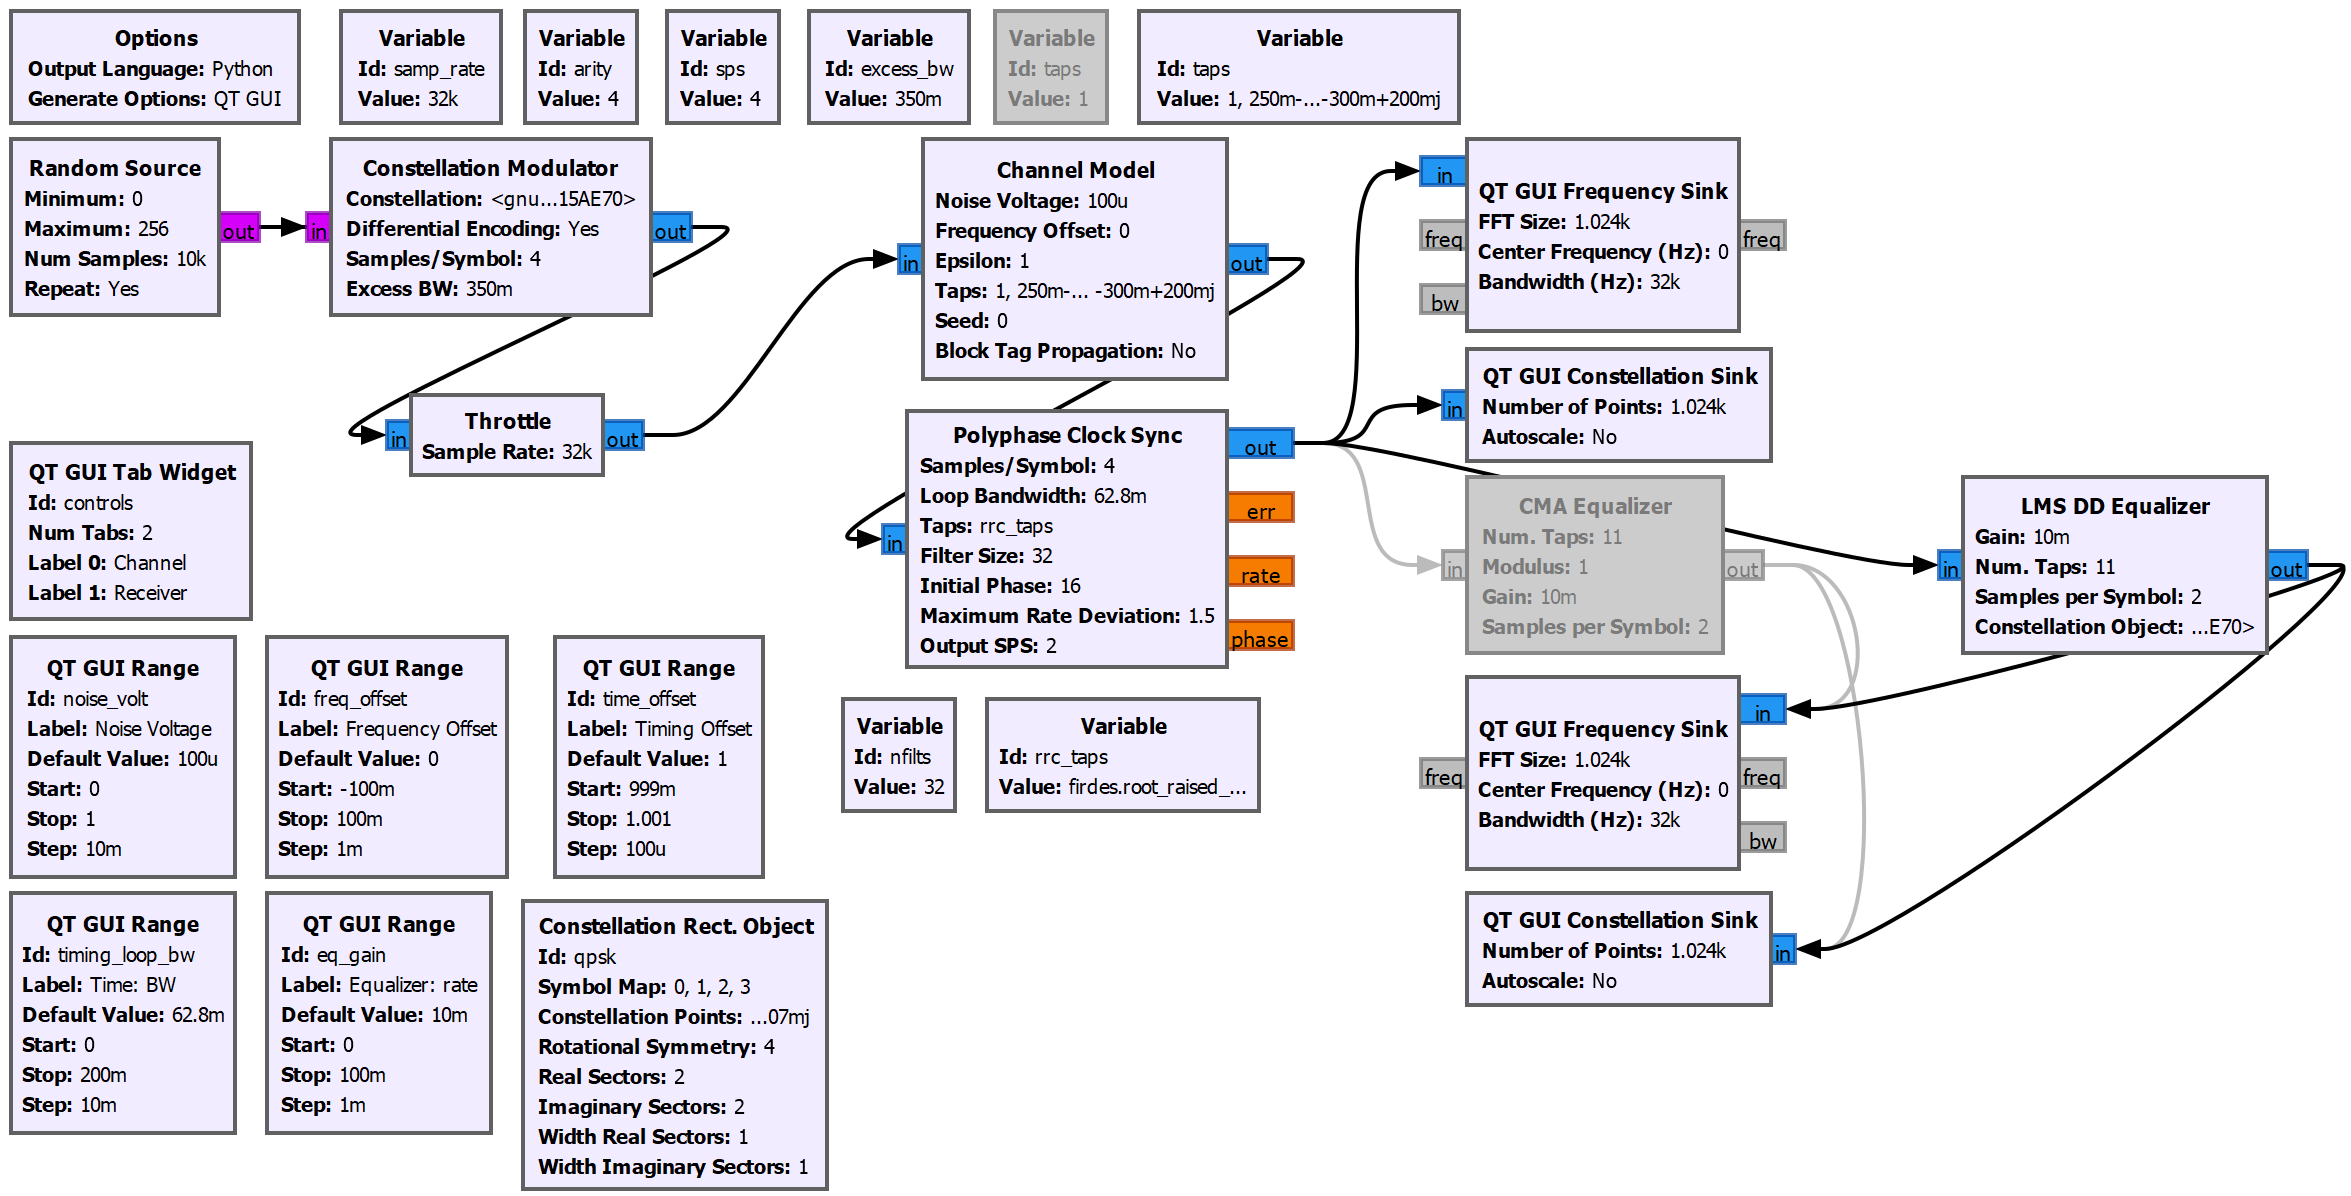
\includegraphics[width=1.0\textwidth]{lab12_fig5_3.png}
        \caption{mpsk\_stage4 граф с \texttt{DD LMS}}
        \label{fig:lab12_fig5_3}
\end{figure}

\chapter{Фазовая и точная частотная коррекция}

Учитывая, что мы выровняли канал, у нас всё ещё есть проблема смещения фазы и частоты. Эквалайзеры, как правило, не адаптируются быстро, поэтому смещение частоты может быть легко за пределами возможностей эквалайзера. Кроме того, если мы просто запускаем эквалайзер \texttt{CMA}, всё, о чем он заботится, - это схождение к единичной окружности. Он ничего не знает о созвездии, поэтому, когда он блокируется, он блокируется на любой заданной фазе. Теперь нам нужно исправить любой сдвиг фазы, а также любой сдвиг частоты.

Для этой задачи мы собираемся использовать \texttt{Costas Loop} в примере. Блок \texttt{Costas Loop} может синхронизировать \texttt{BPSK}, \texttt{QPSK} и \texttt{8PSK}. Приёмник созвездия будет привязан к любому заданному объекту созвездия, хотя в зависимости от созвездия функция принятия решения может быть более или менее сложной.

\begin{figure}[H]
        \centering
        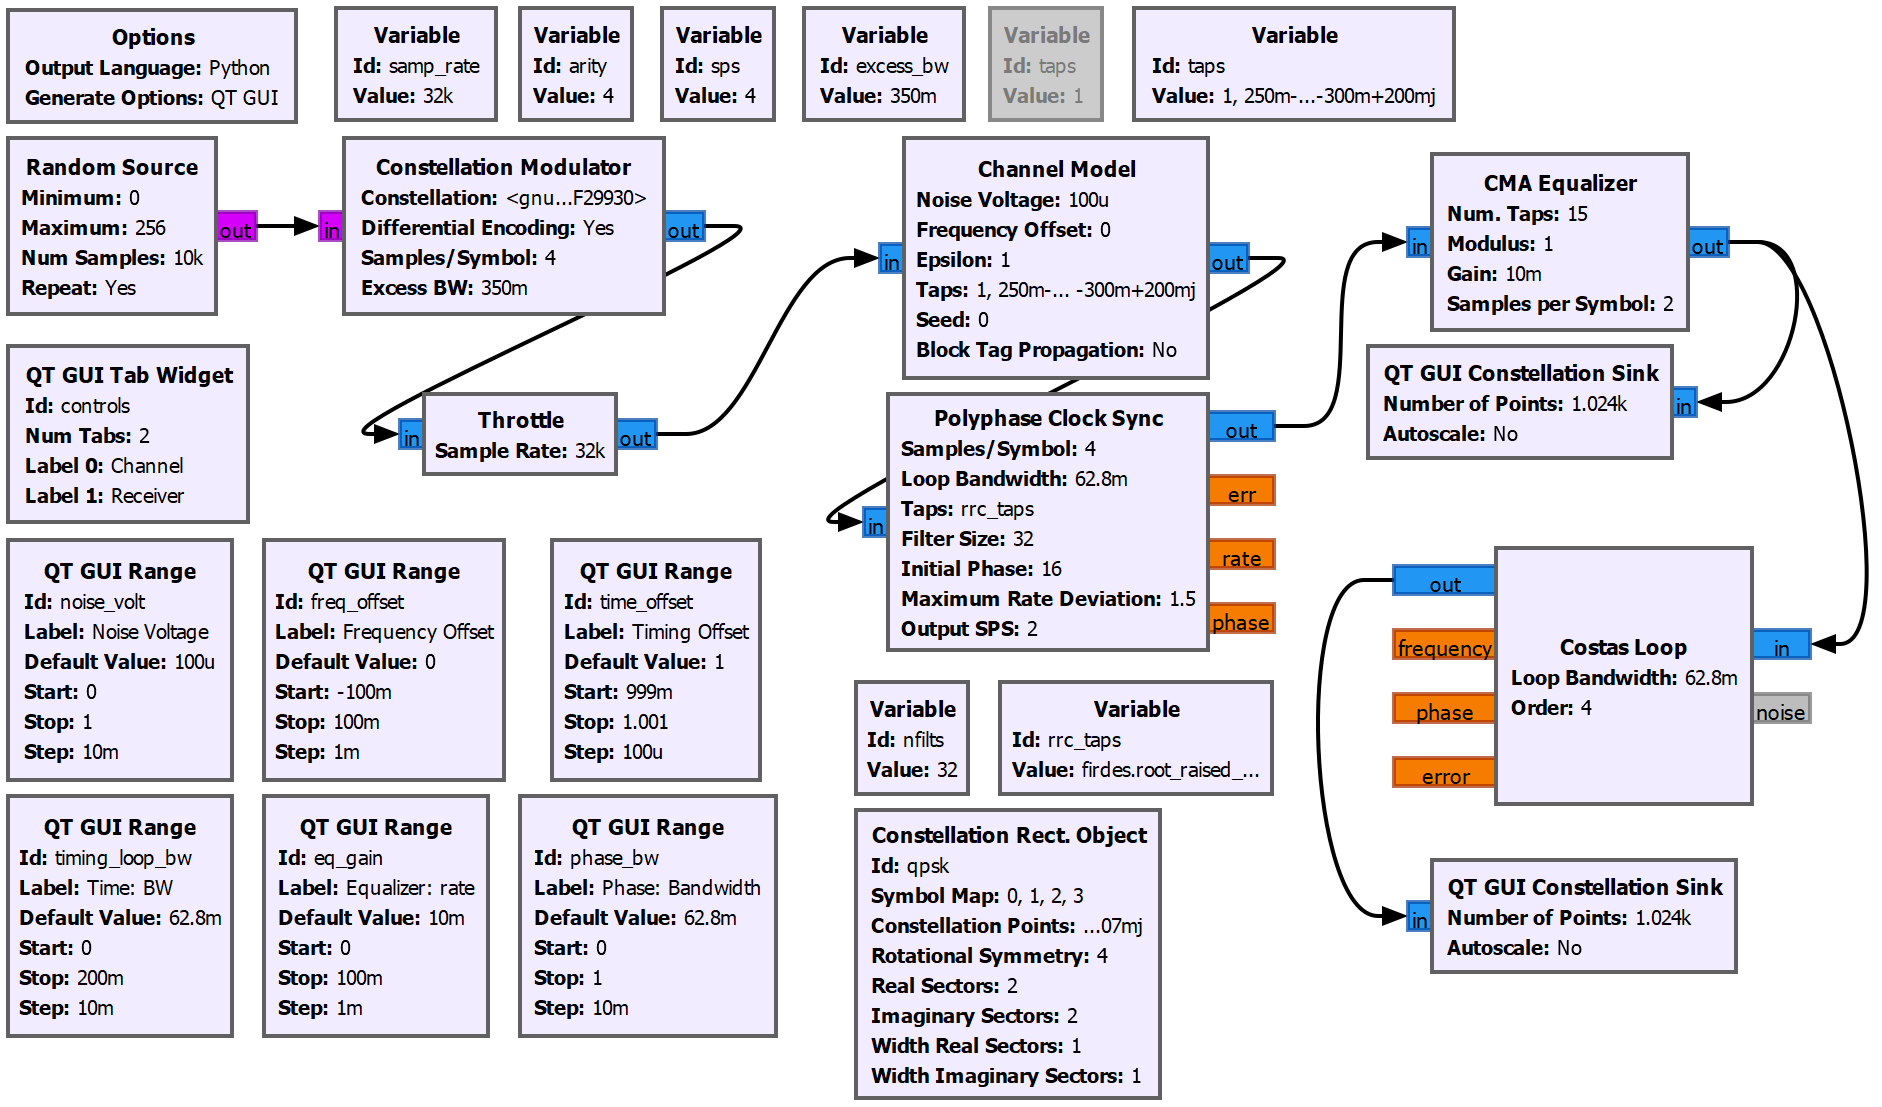
\includegraphics[width=1.0\textwidth]{lab12_fig6_1.png}
        \caption{mpsk\_stage5 граф}
        \label{fig:lab12_fig6_1}
\end{figure}

Установим шум, временной сдвиг, простой многолучевой канал и частотный сдвиг. После эквалайзера мы видим, что все символы находятся на единичном круге, но вращаются из-за сдвига частоты, который еще ничего не исправляет. На выходе блока \texttt{Costas Loop} мы можем видеть заблокированное созвездие, как мы начали, плюс дополнительный шум, с которым мы ничего не можем поделать.

\begin{figure}[H]
        \centering
        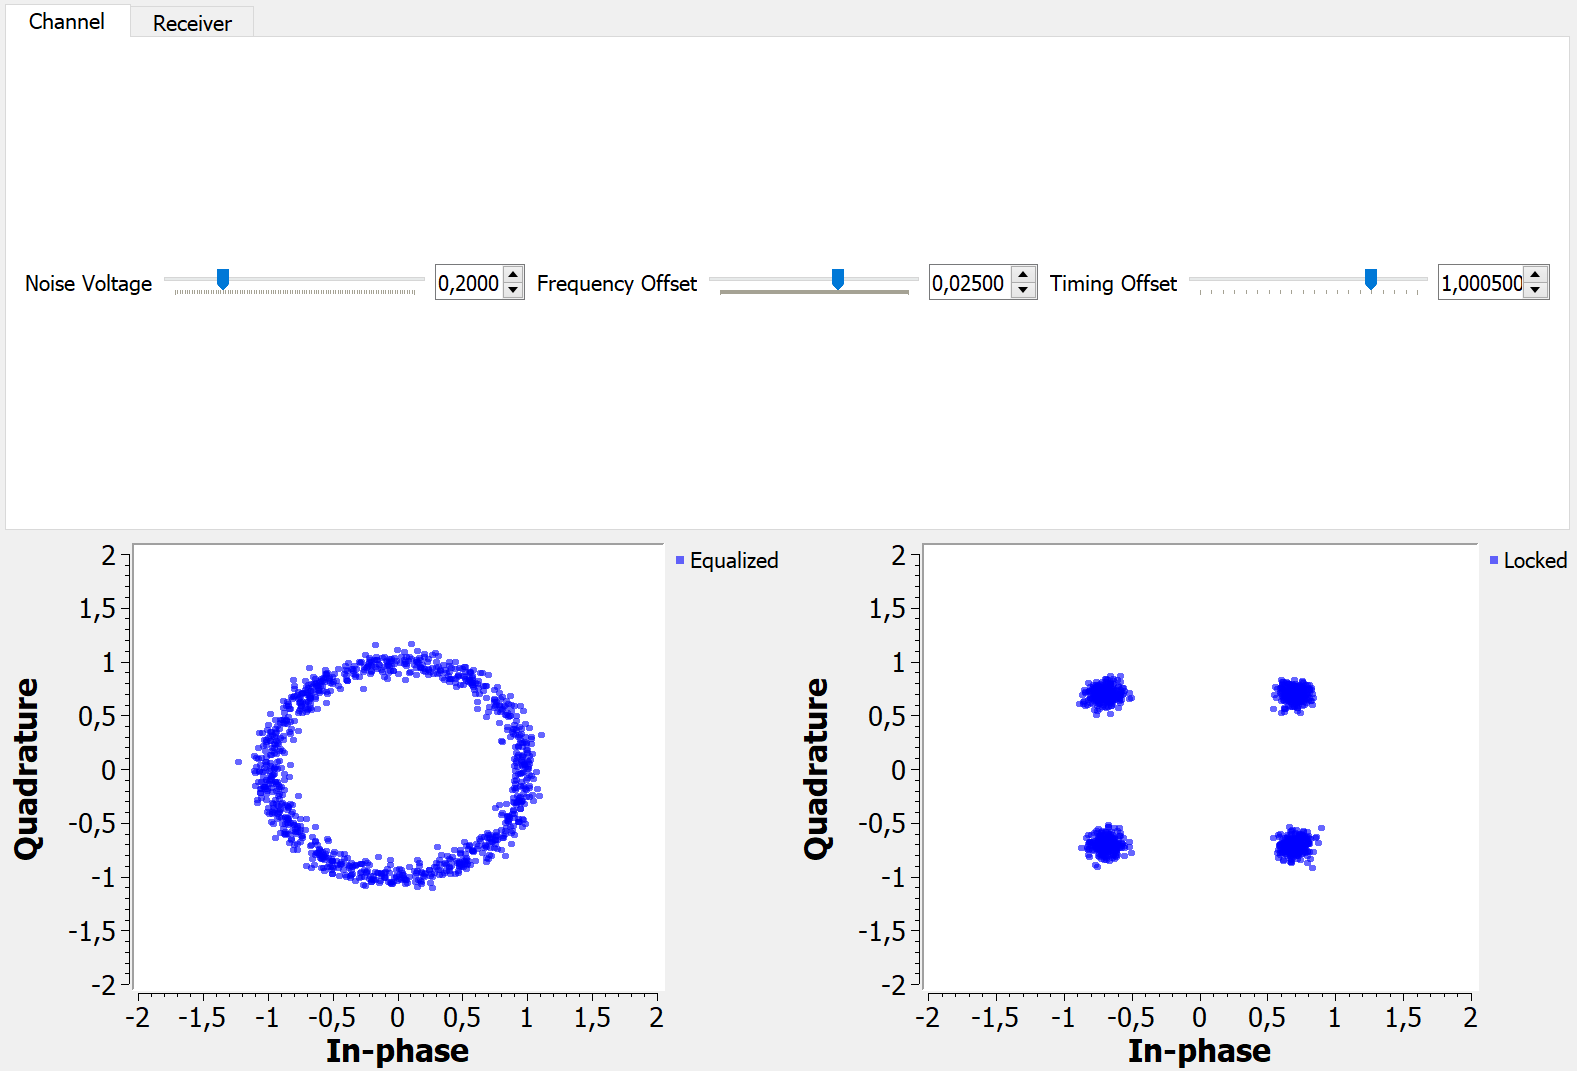
\includegraphics[width=1.0\textwidth]{lab12_fig6_2.png}
        \caption{Визуализация данных графа}
        \label{fig:lab12_fig6_2}
\end{figure}

\chapter{Декодирование}

Теперь мы можем декодировать сигнал. Для этого мы вставляем \texttt{Constellation Decoder} после \texttt{Costas Loop}, а также изменяем параметр \texttt{Differential} в блоке \texttt{Constellation Modulator} значение на False.

\begin{figure}[H]
        \centering
        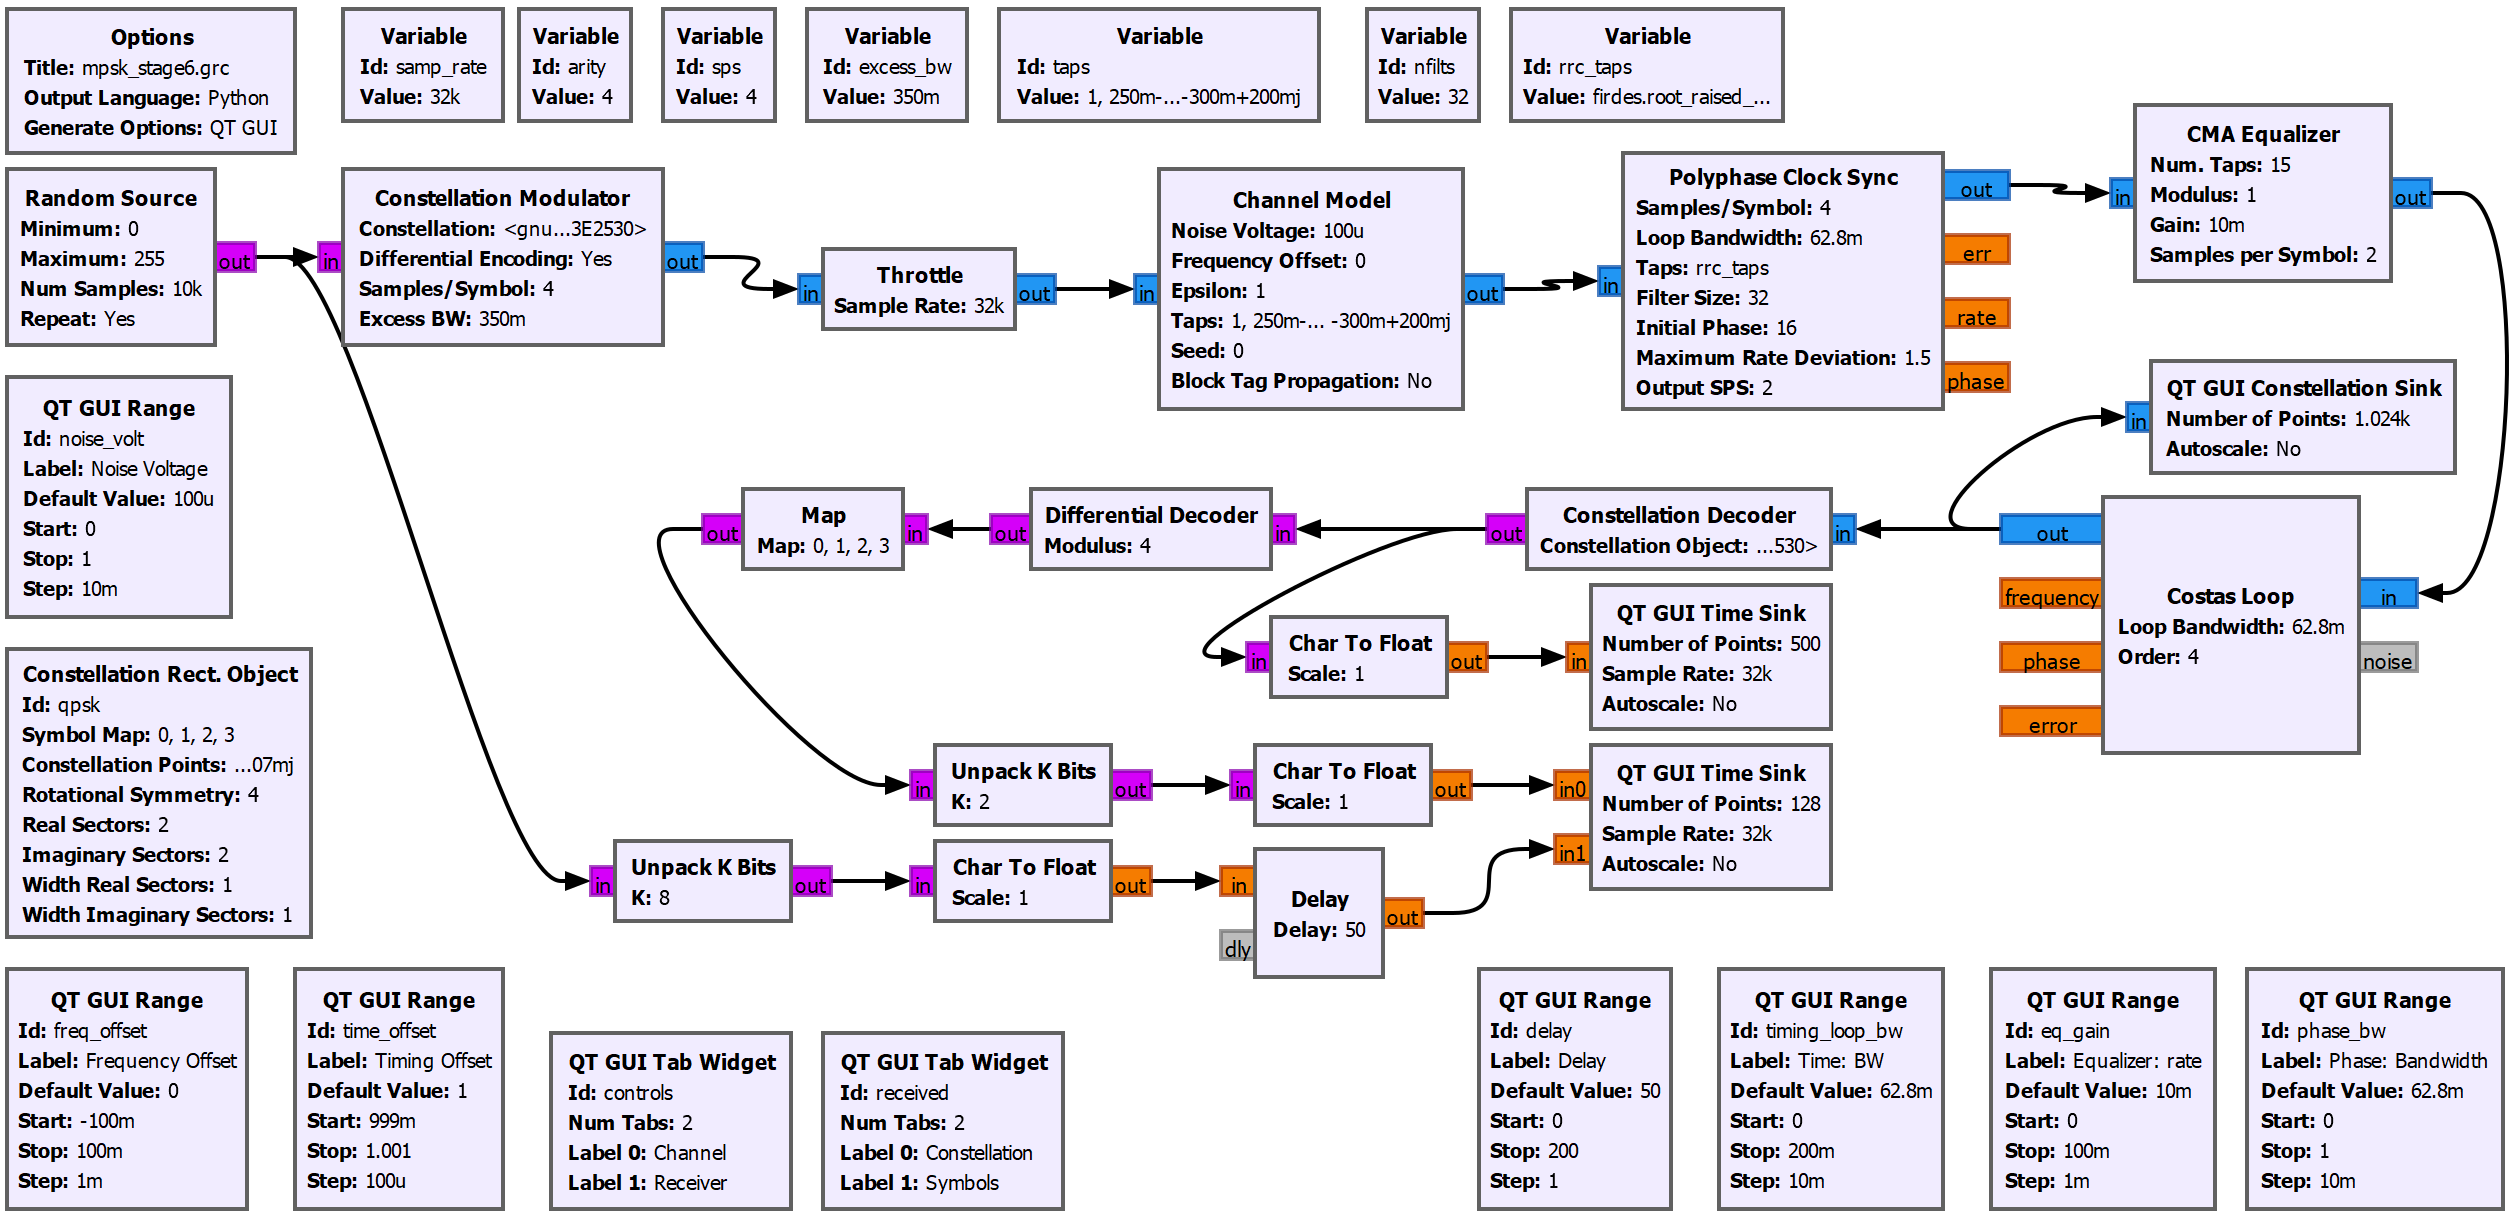
\includegraphics[width=1.0\textwidth]{lab12_fig7_1.png}
        \caption{mpsk\_stage6 граф}
        \label{fig:lab12_fig7_1}
\end{figure}

 Здесь мы можем настроить задержку, чтобы найти правильное значение и посмотреть, как синхронизируются биты. Вы также можете вычесть один сигнал из другого, чтобы увидеть, когда они синхронизированы, так как на выходе будет 0. Добавление шума и других влияний на канал можно легко увидеть как битовые ошибки, если этот сигнал не равен 0.
 
 \begin{figure}[H]
        \centering
        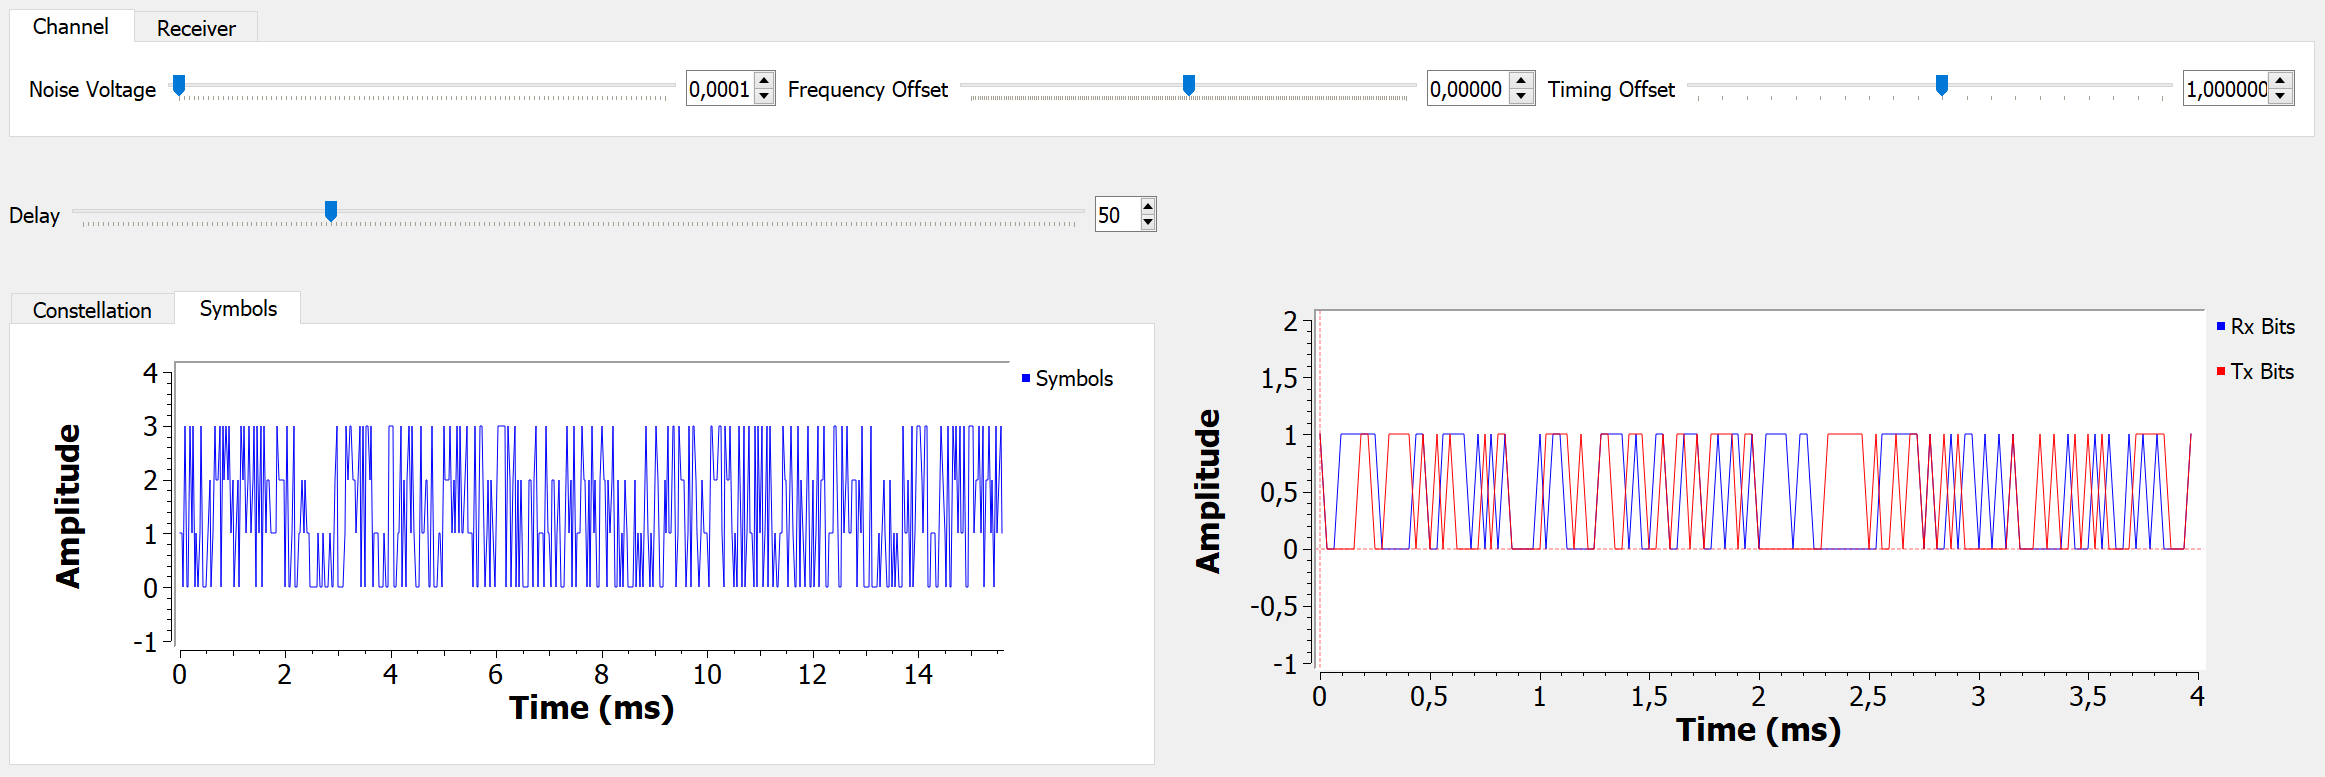
\includegraphics[width=1.0\textwidth]{lab12_fig7_2.png}
        \caption{Визуализация данных графа}
        \label{fig:lab12_fig7_2}
\end{figure}

\chapter{Выводы}

Во время выполнения лабораторной работы получены навыки работы с моделированием, настройки симуляции, а также восстановление сигнала.

\end{document}